\subsection{Human Interface Design}
\subsubsection{Login and Registration Pages}
The registration user interfaces are shown here.
\begin{center}
\begin{tabular}{ccc}
    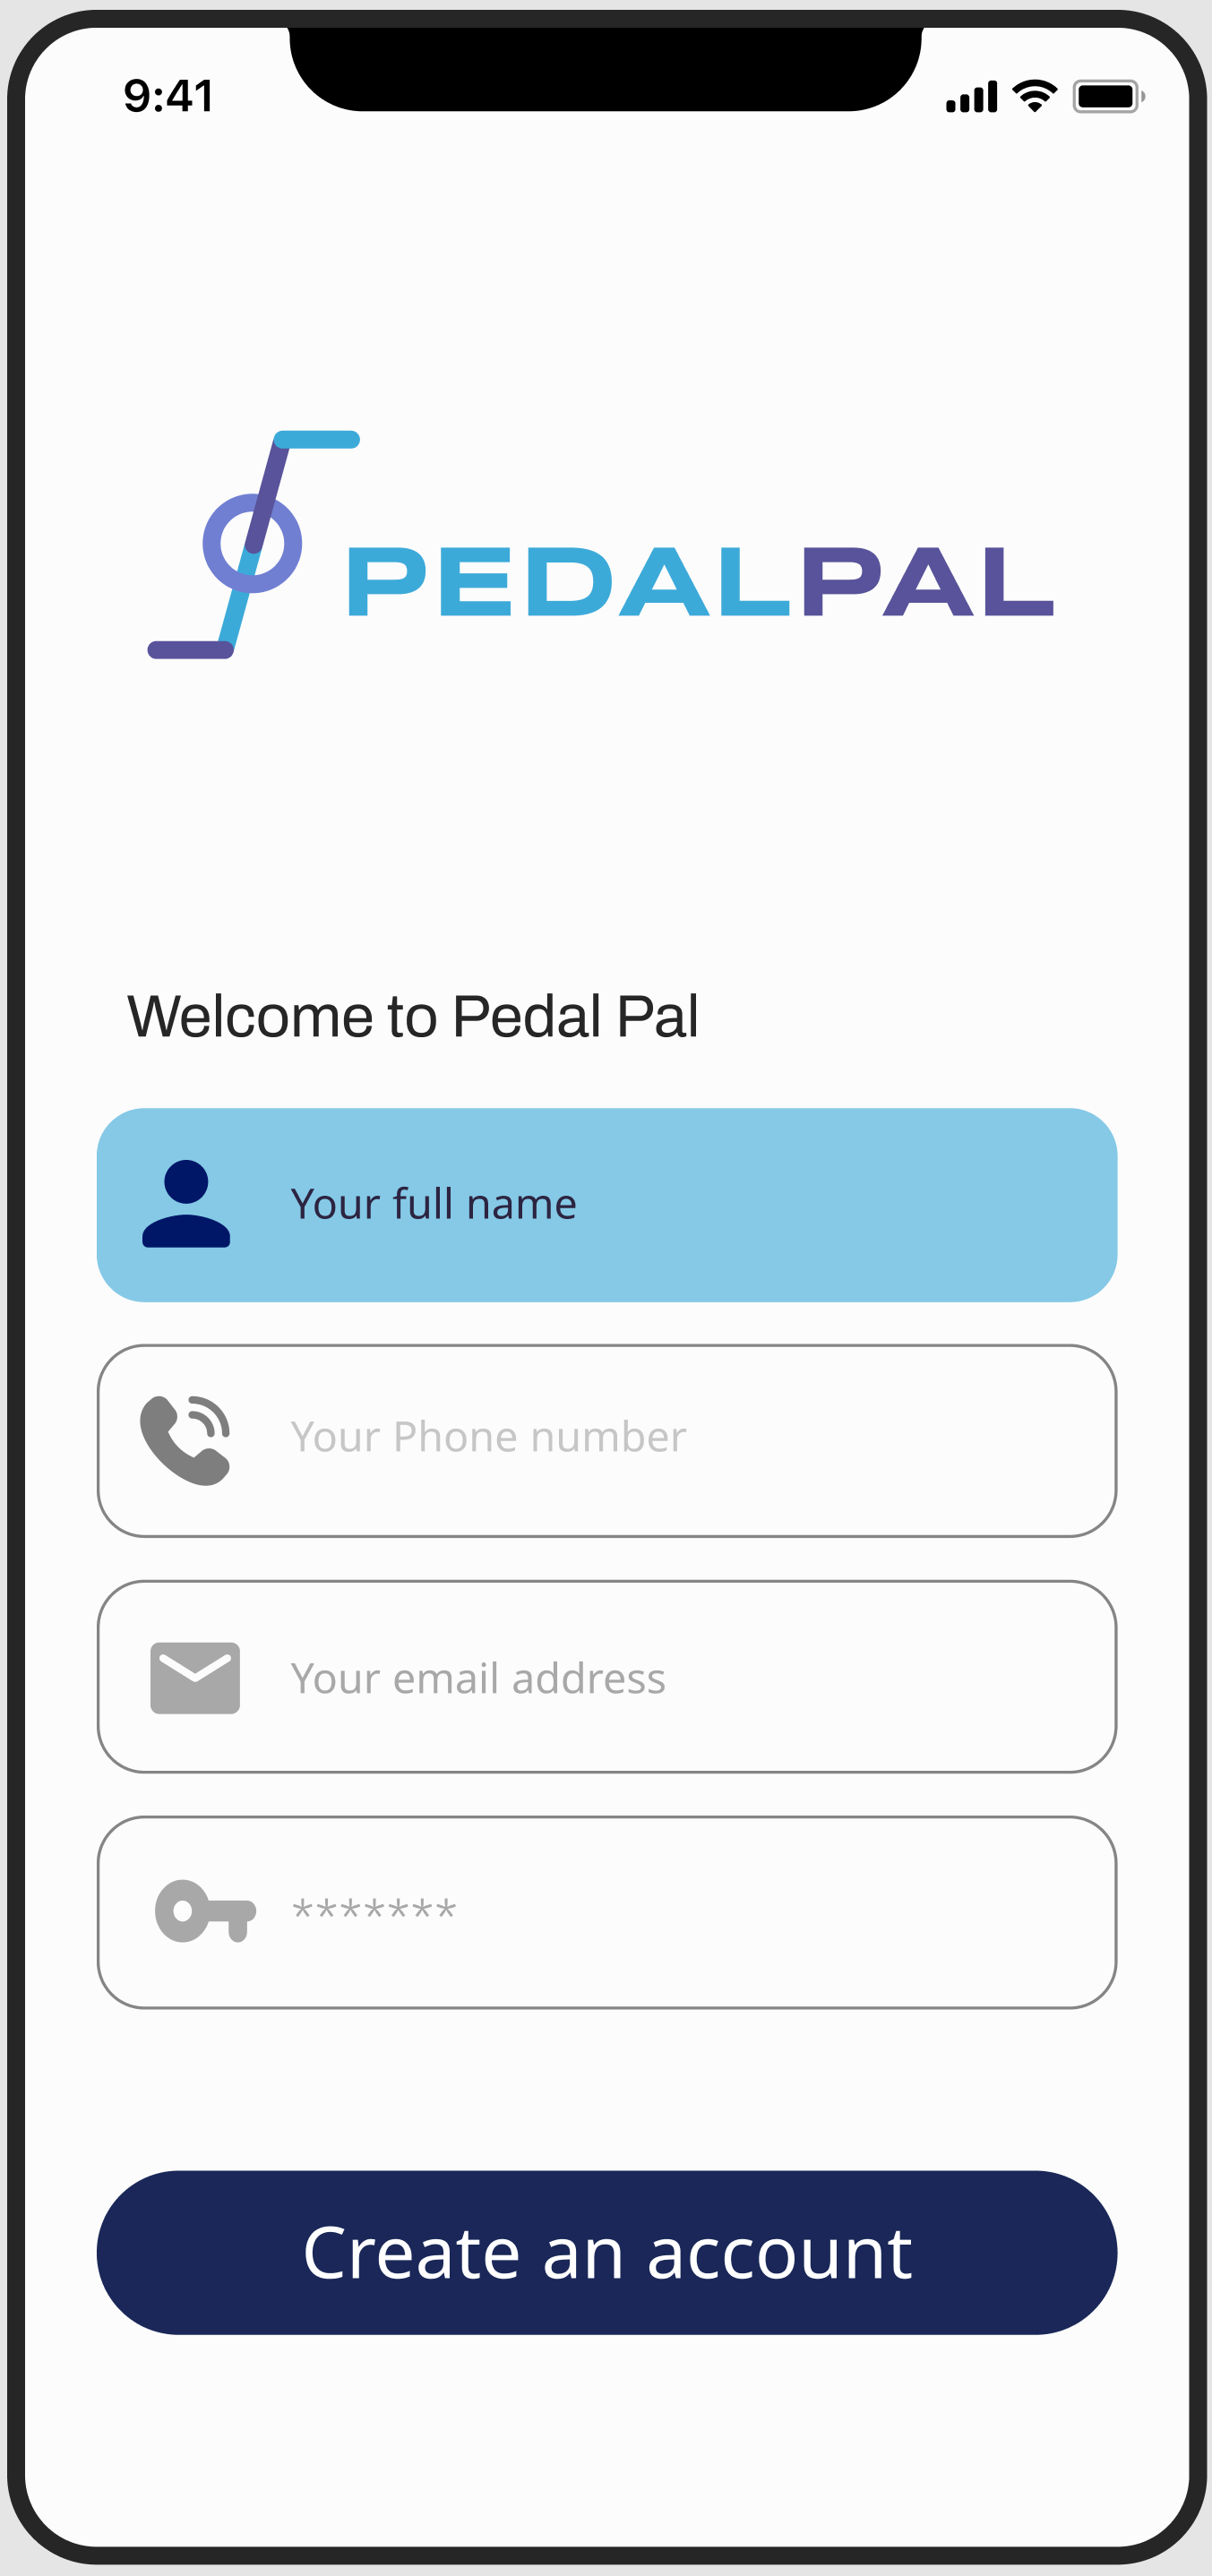
\includegraphics[scale=0.1]{ui-images/Register.png} & 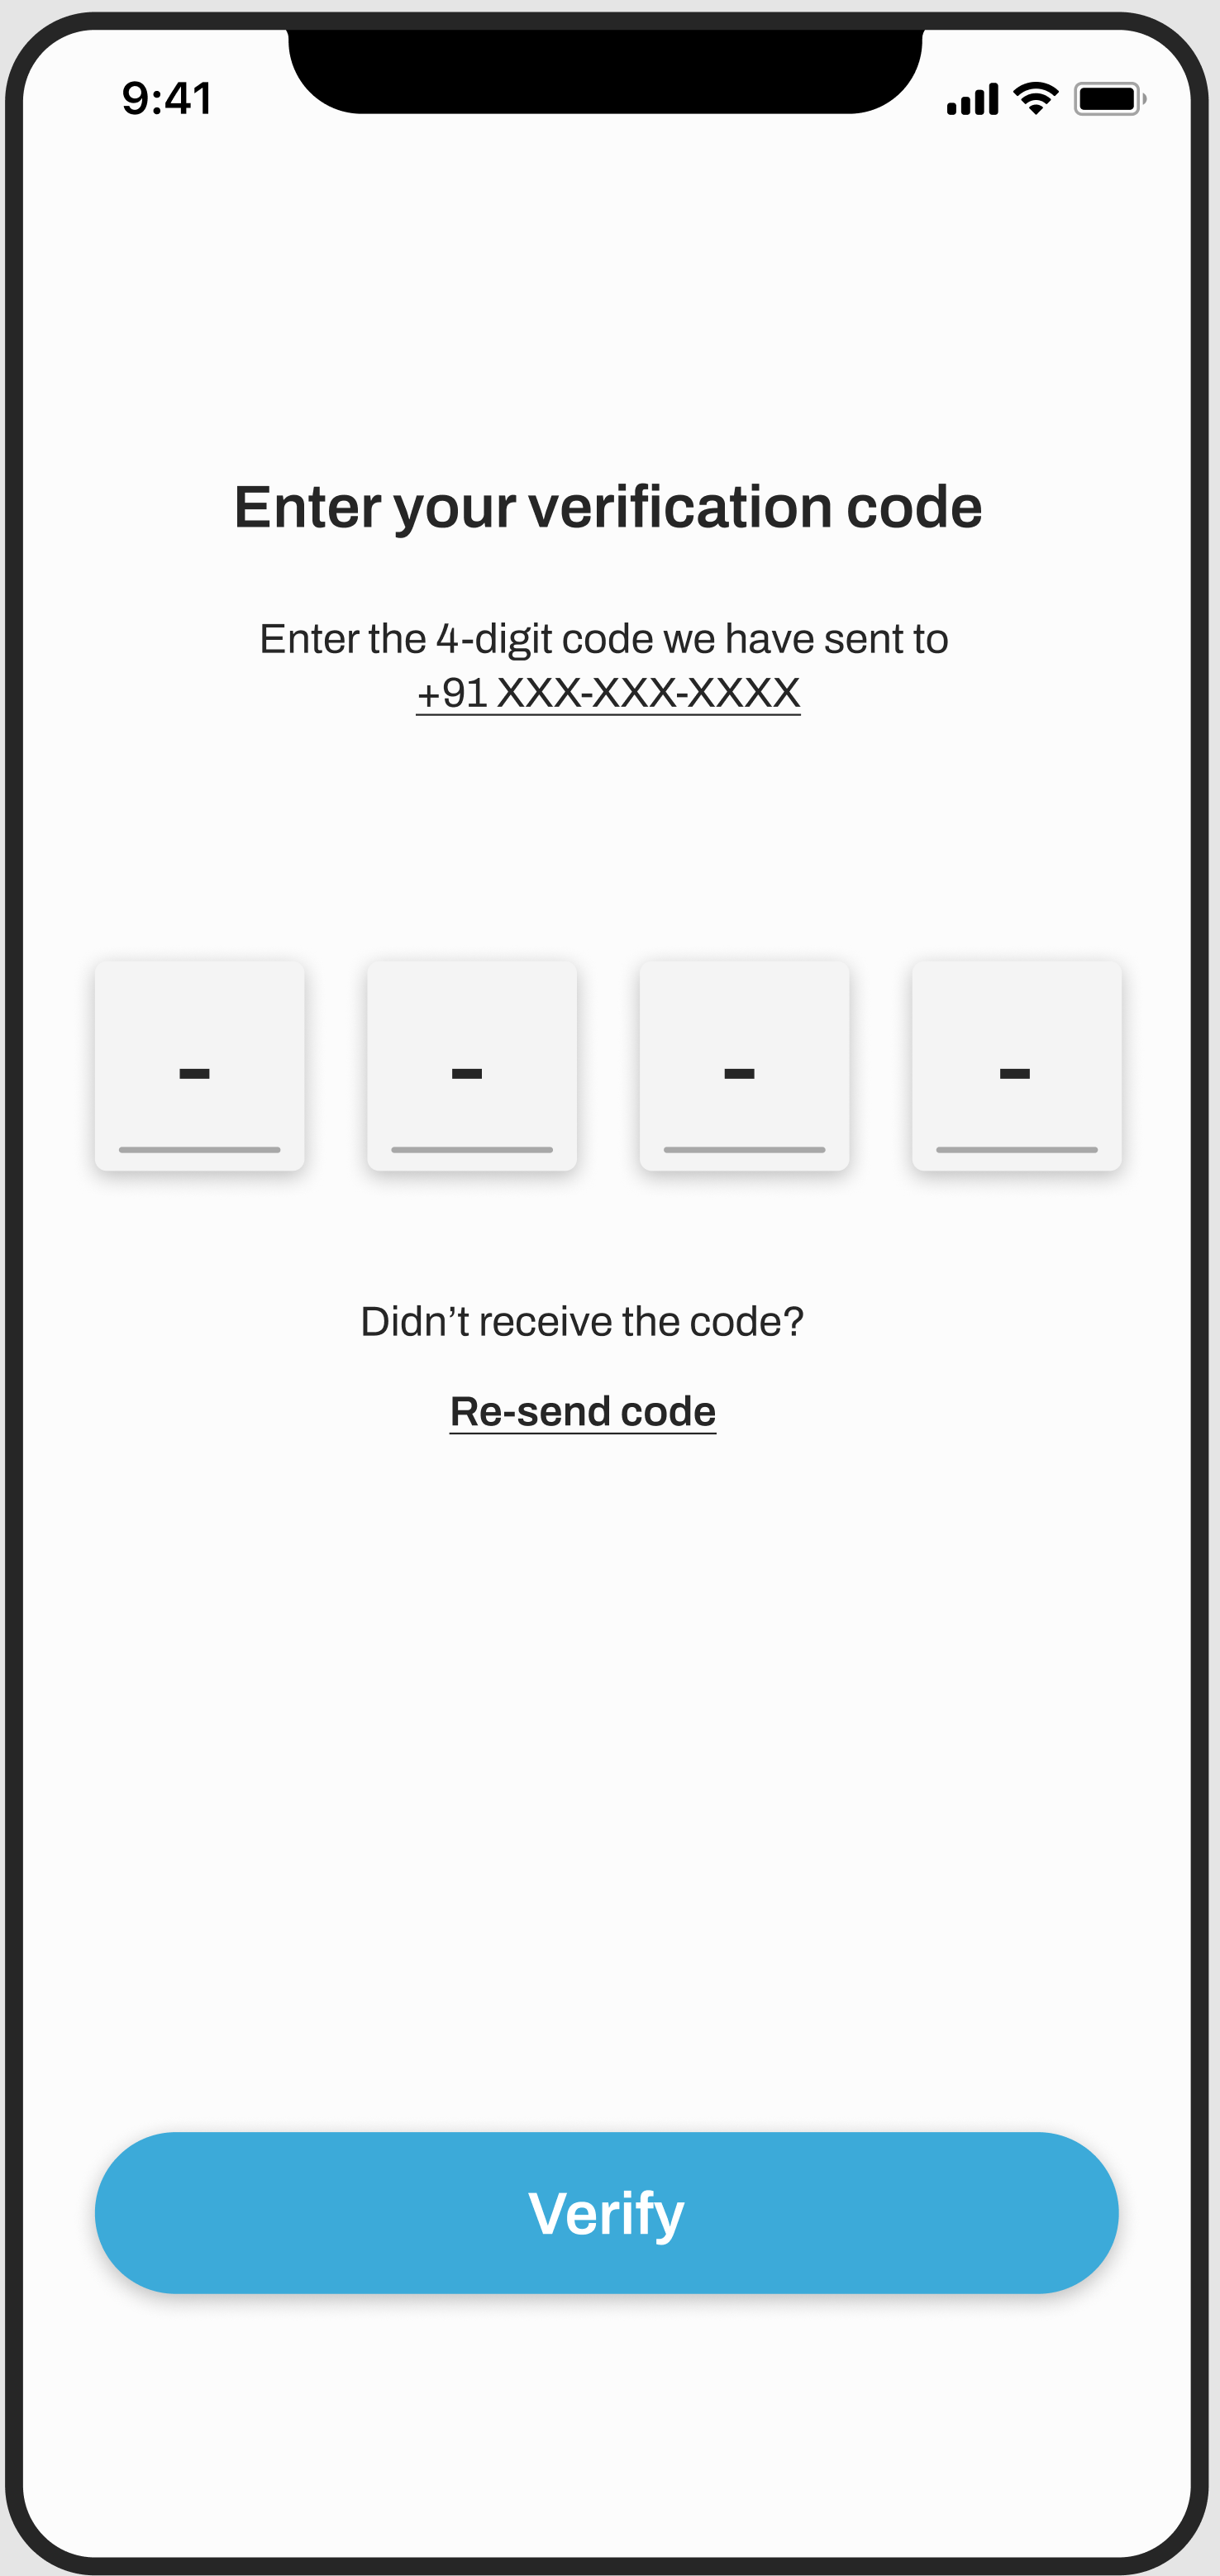
\includegraphics[scale=0.1]{ui-images/PhoneOTP.png} &    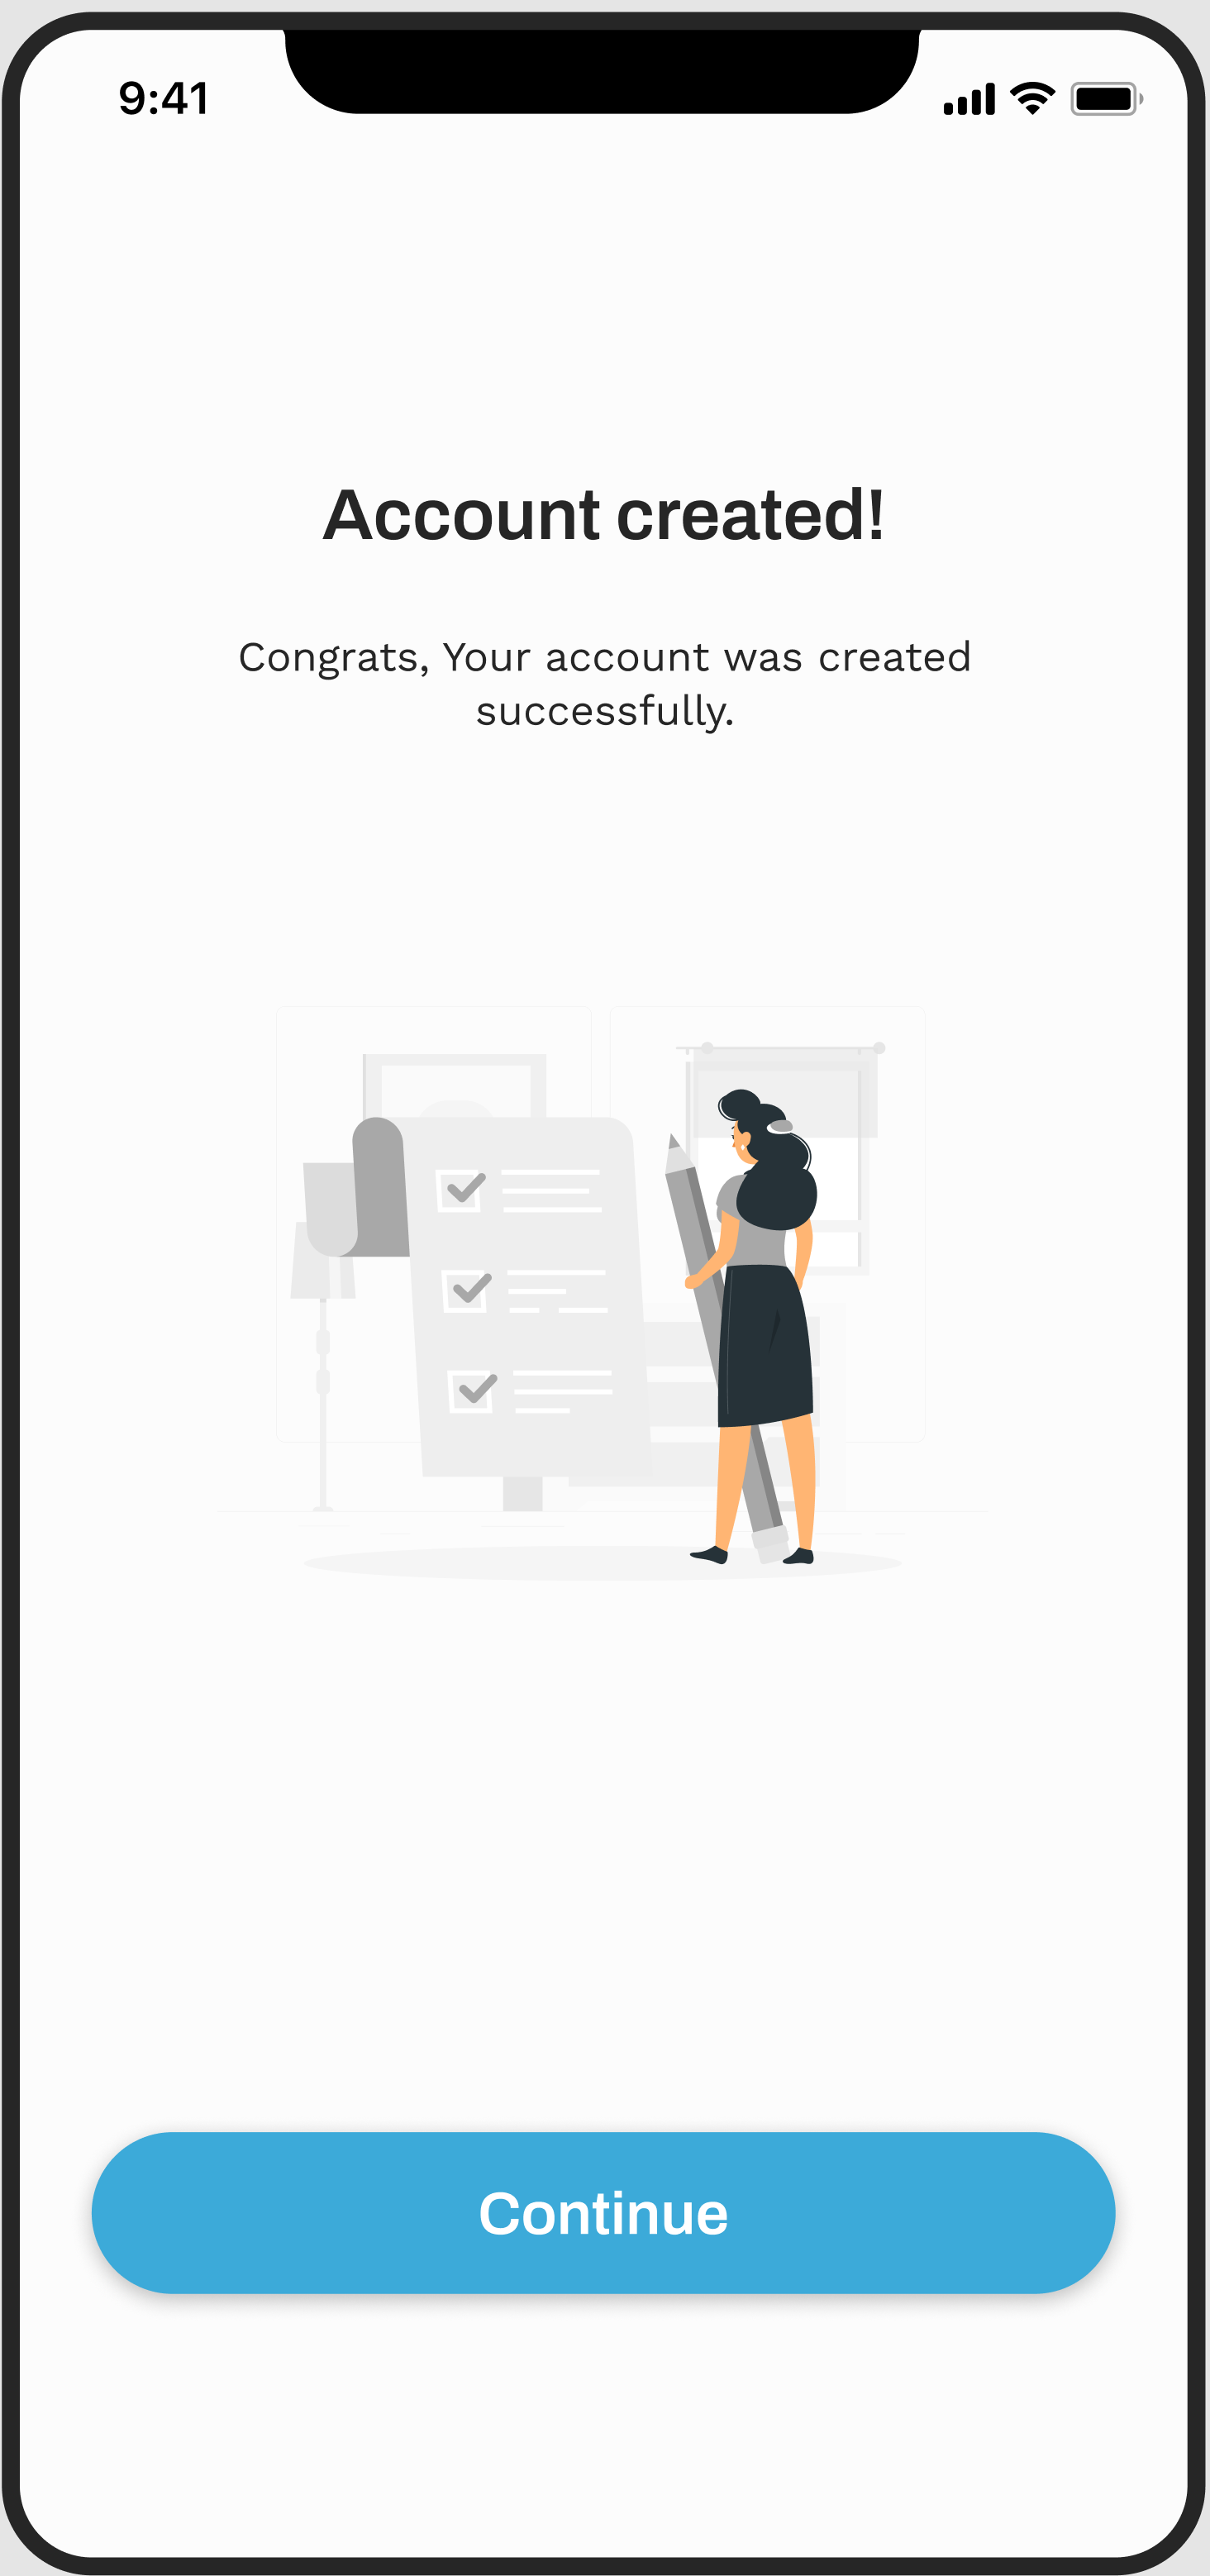
\includegraphics[scale=0.1]{ui-images/AccountSuccess.png}
\end{tabular}
\end{center}
The login workflow is shown here. If the user has not created an account yet, they can click on Sign Up to create a new accout. If the user has forgotten their password, they can reset it using the "Forgot Password" button.
\begin{center}
\begin{tabular}{ccc}
    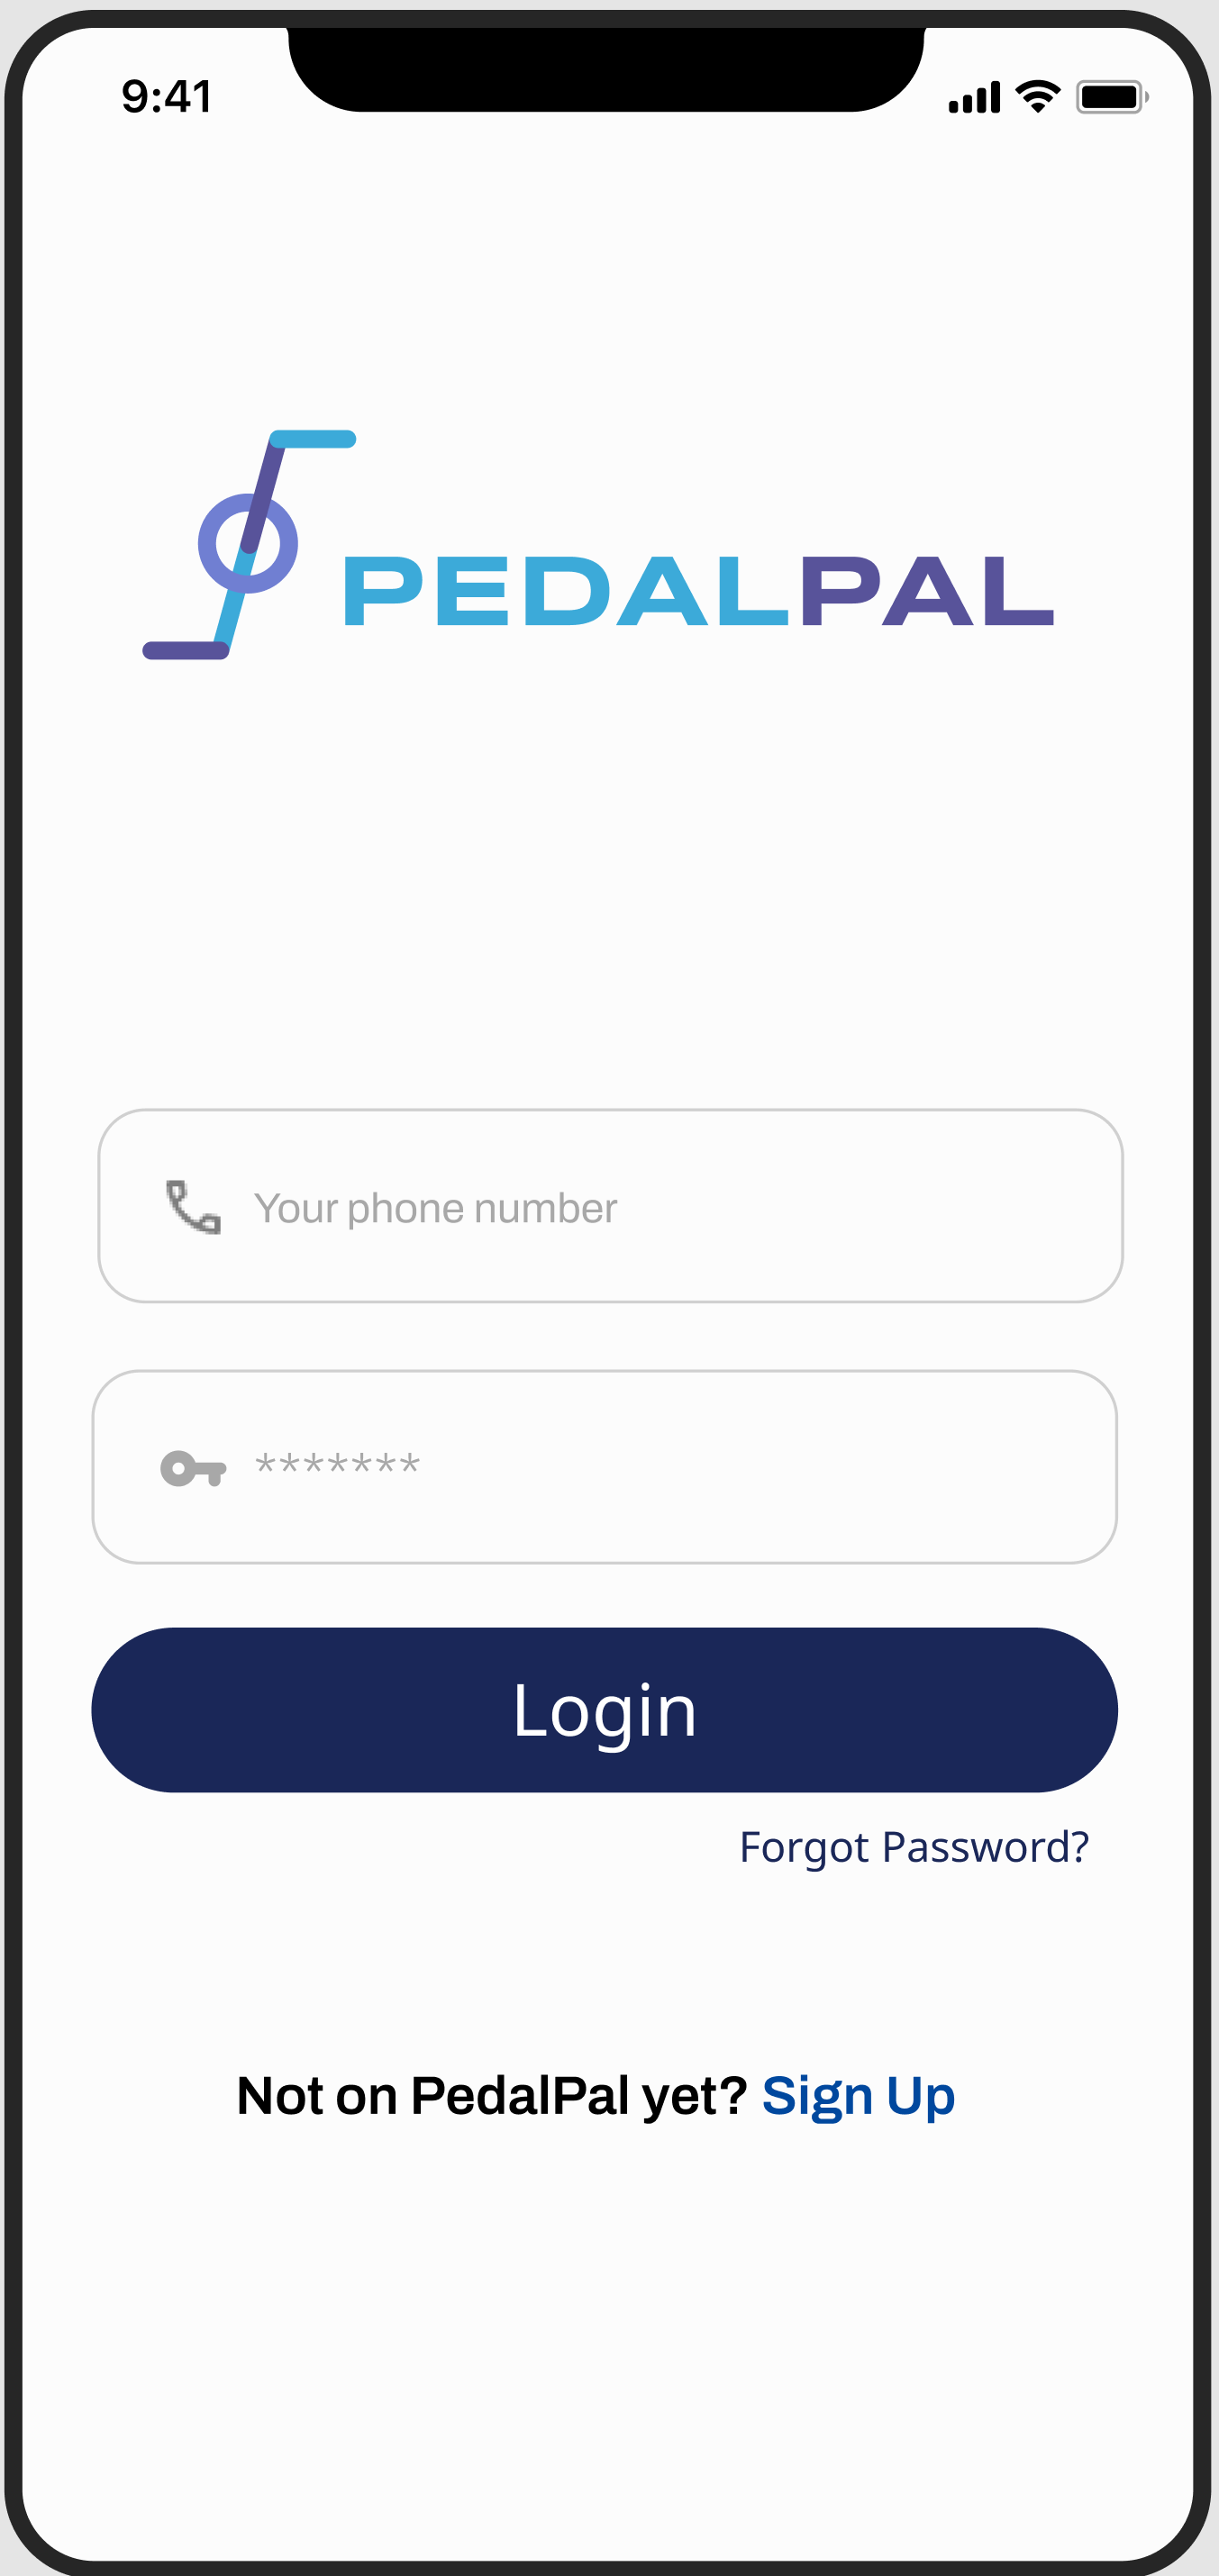
\includegraphics[scale=0.1]{ui-images/Login.png} & 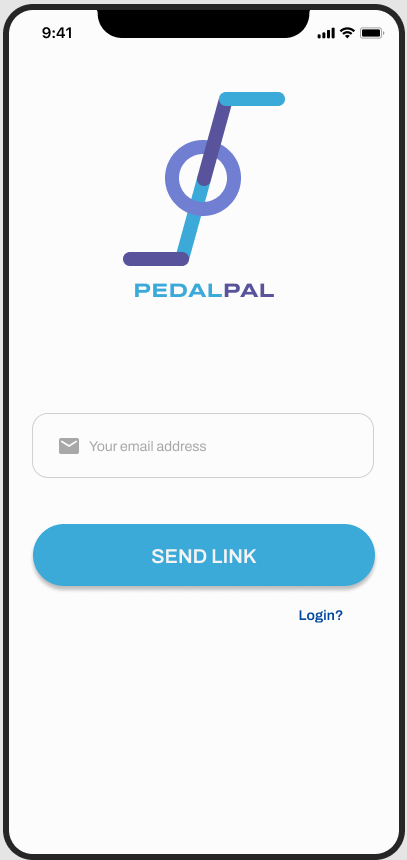
\includegraphics[scale=0.1]{ui-images/EmailOTP.png} &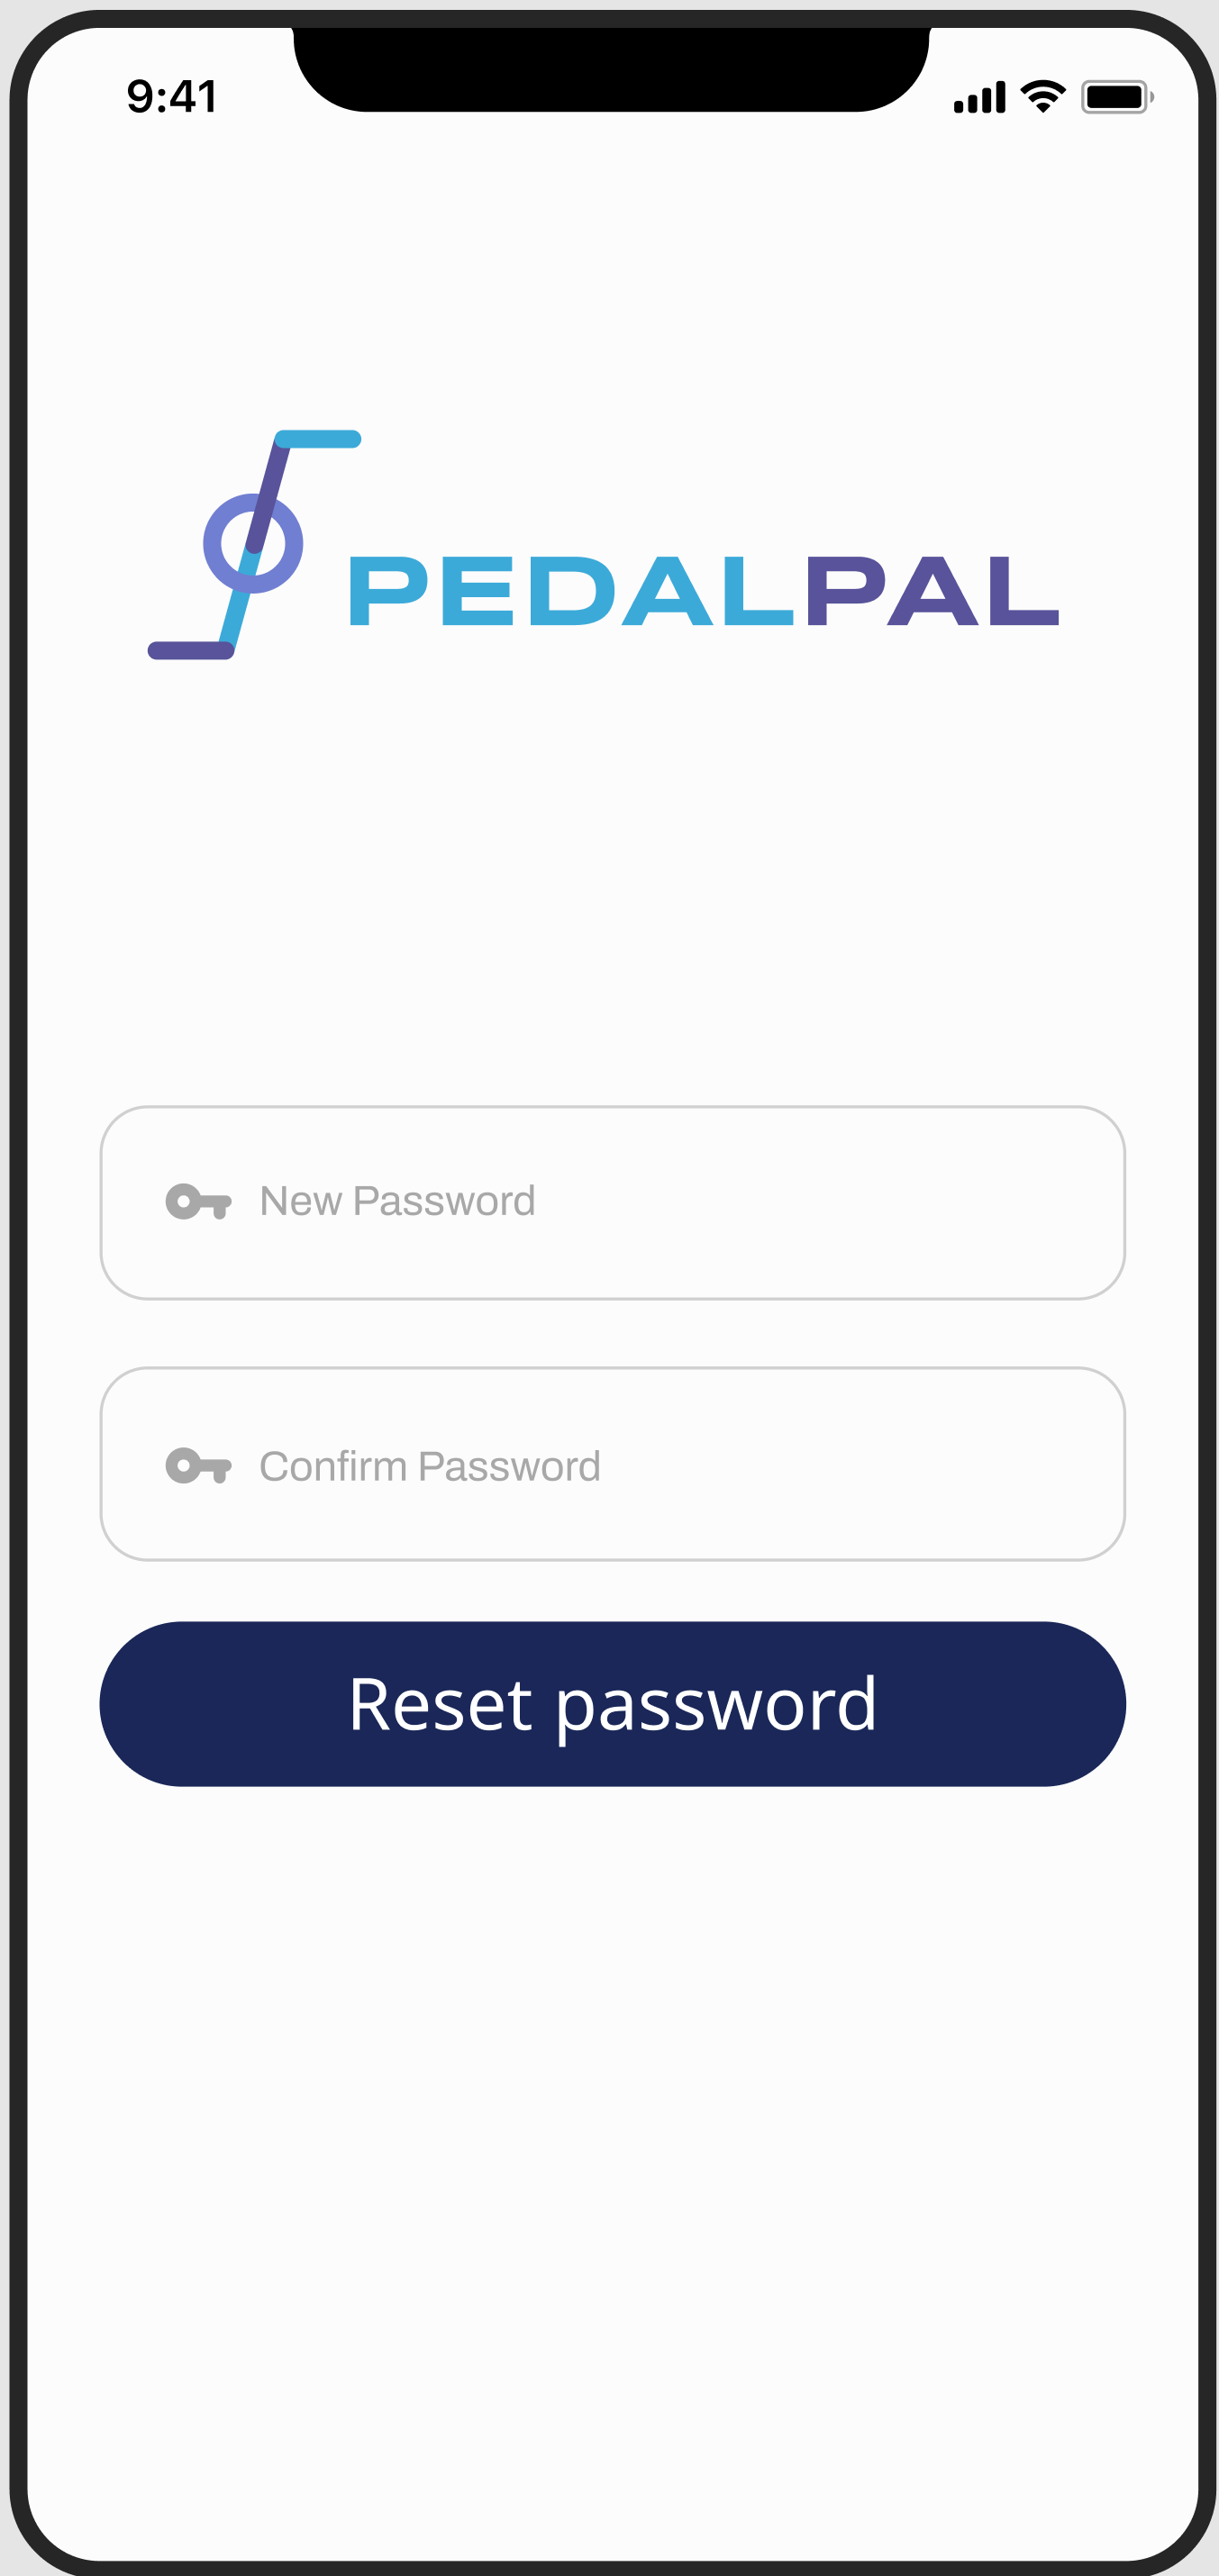
\includegraphics[scale=0.1]{ui-images/ResetPassword.png}
\end{tabular}
\end{center}

\subsubsection{Booking a Ride}
The user sees a map which shows the location of the user along with the hubs present. They can either choose the hub on their map, or search it from the search box. Once a hub is selected, the details of the hub are displayed, including the number of available cycles. The user can choose to start a ride instantly, or book a cycle for a later time (available only for subscribed users). If the user wishes to book for later, they are presented with a time picker. If the user wishes to ride instantly, they are presented with a QR code which they can scan to unlock the cycle. During the ride, statistics like ride time and current cost are shown to the user. Once the ride is over, the user can end the ride and the app will show the user the fare for the ride, and ask for feedback. The user can also report any issues with the cycle during the ride.
\begin{center}
\begin{tabular}{ccc}
    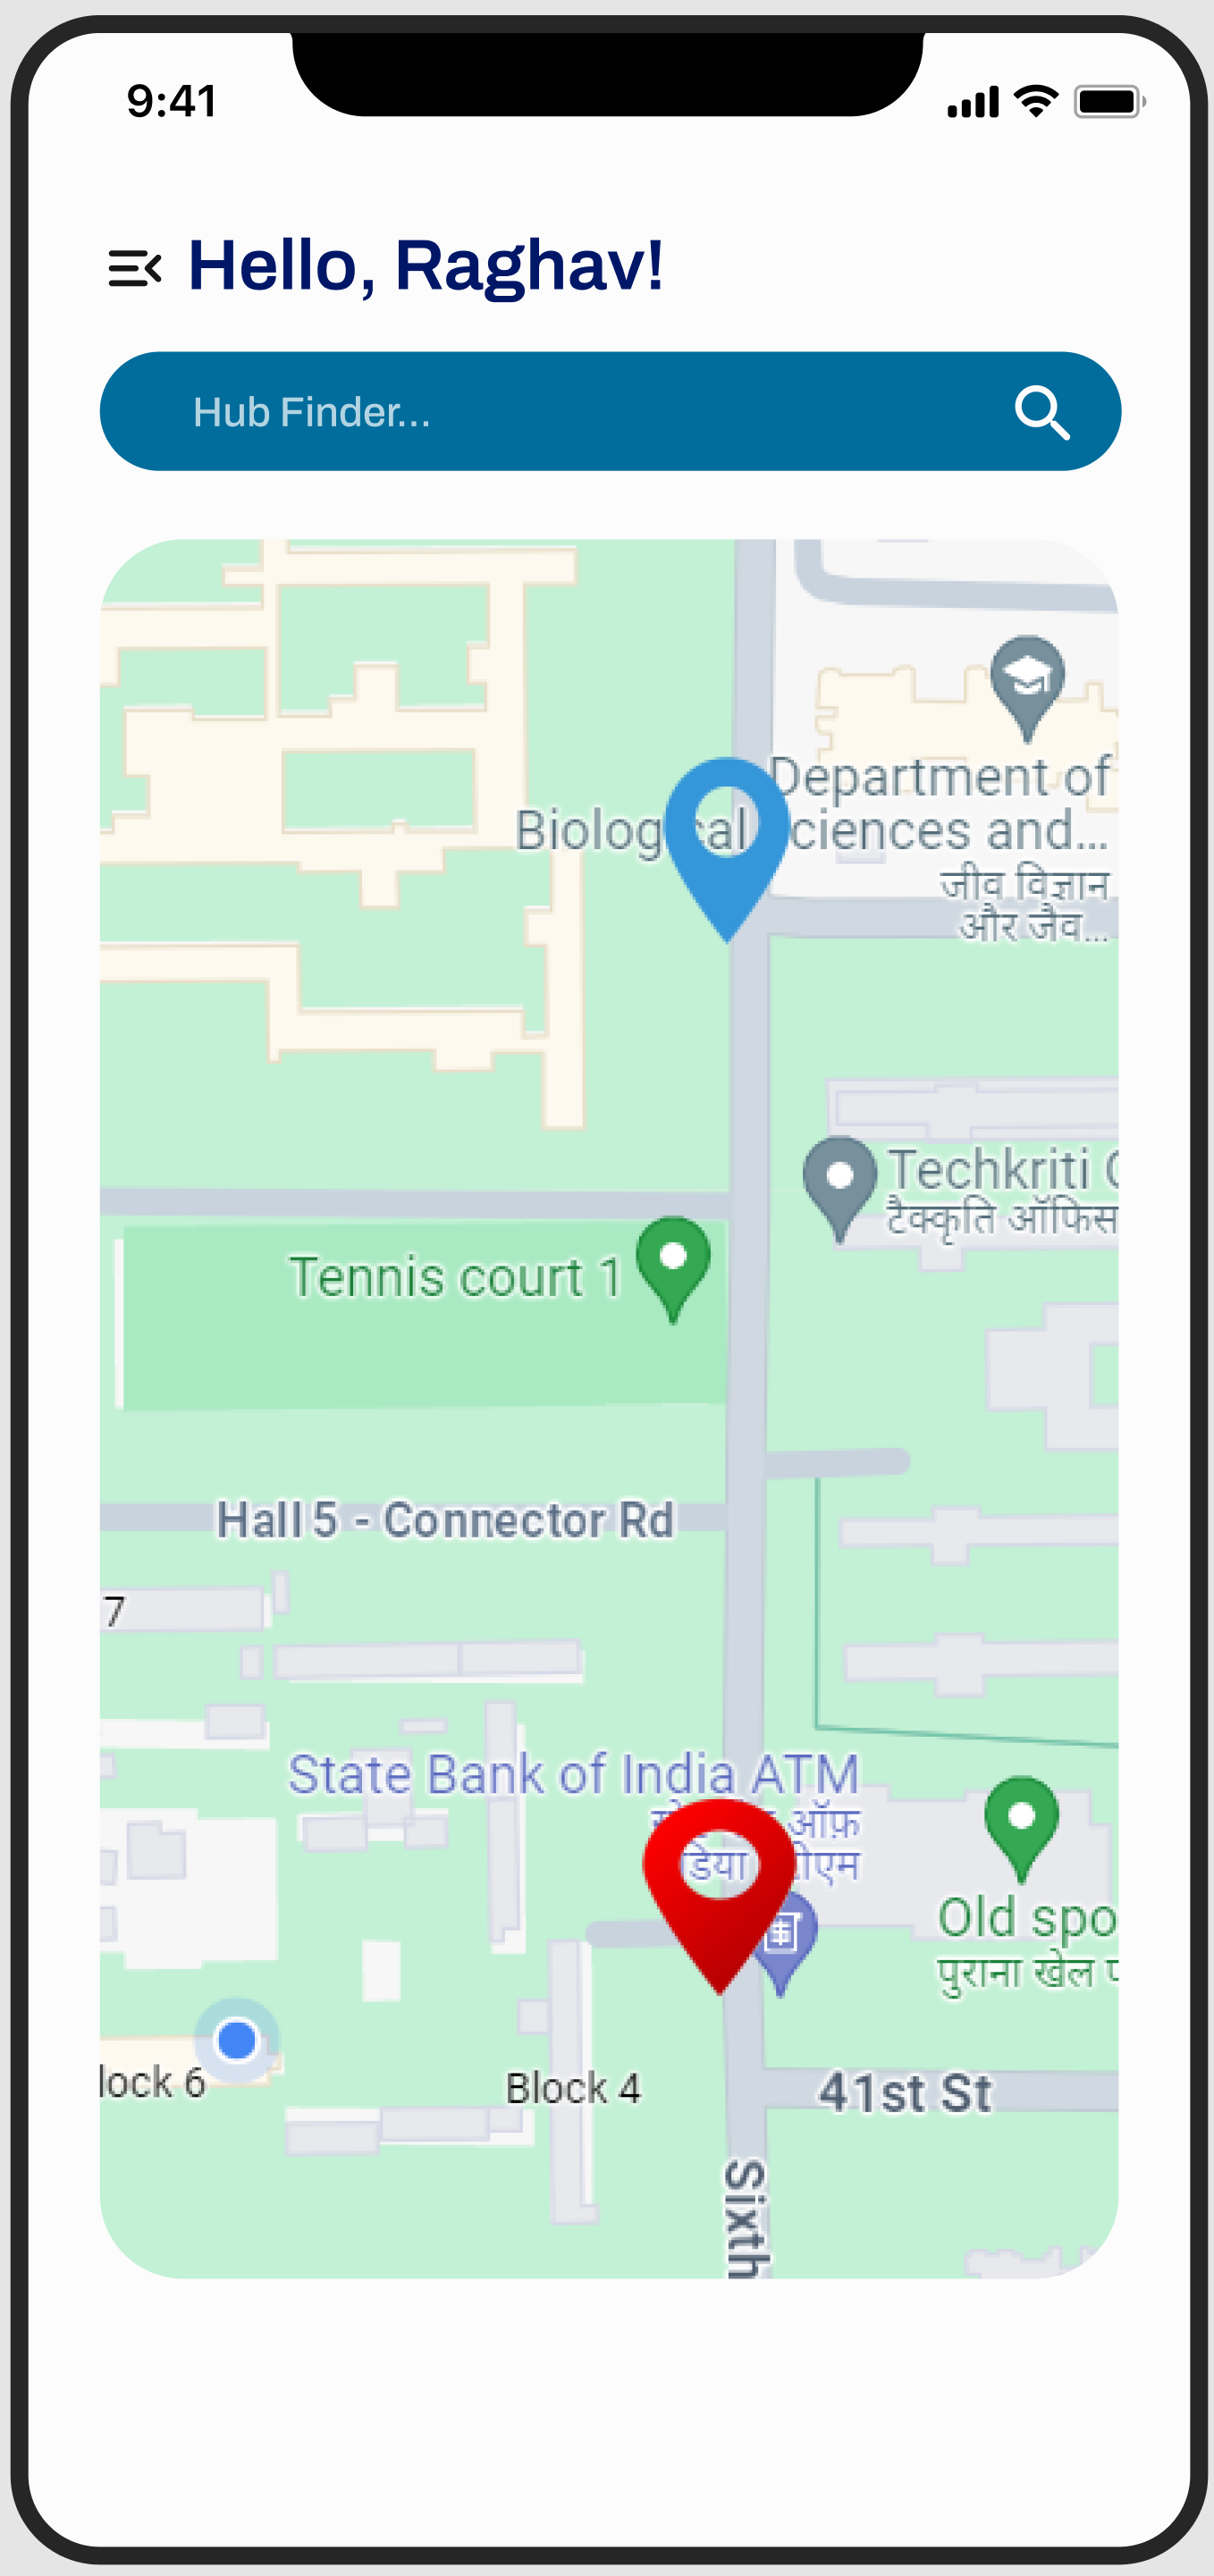
\includegraphics[scale=0.1]{ui-images/Dashboard.png} &
    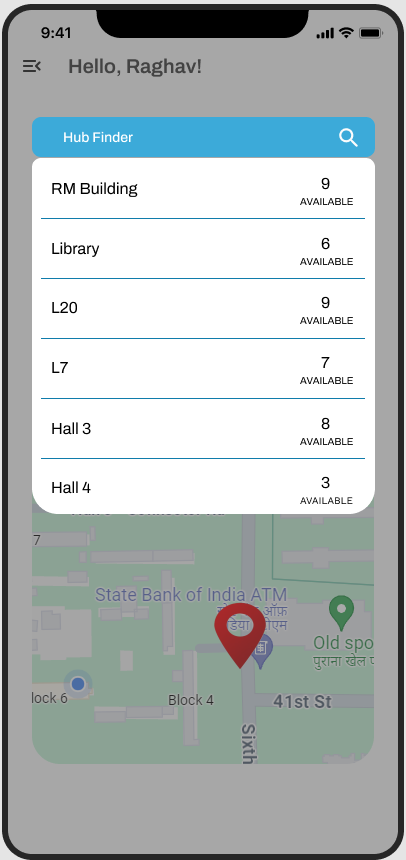
\includegraphics[scale=0.1]{ui-images/HubSelection.png} &
    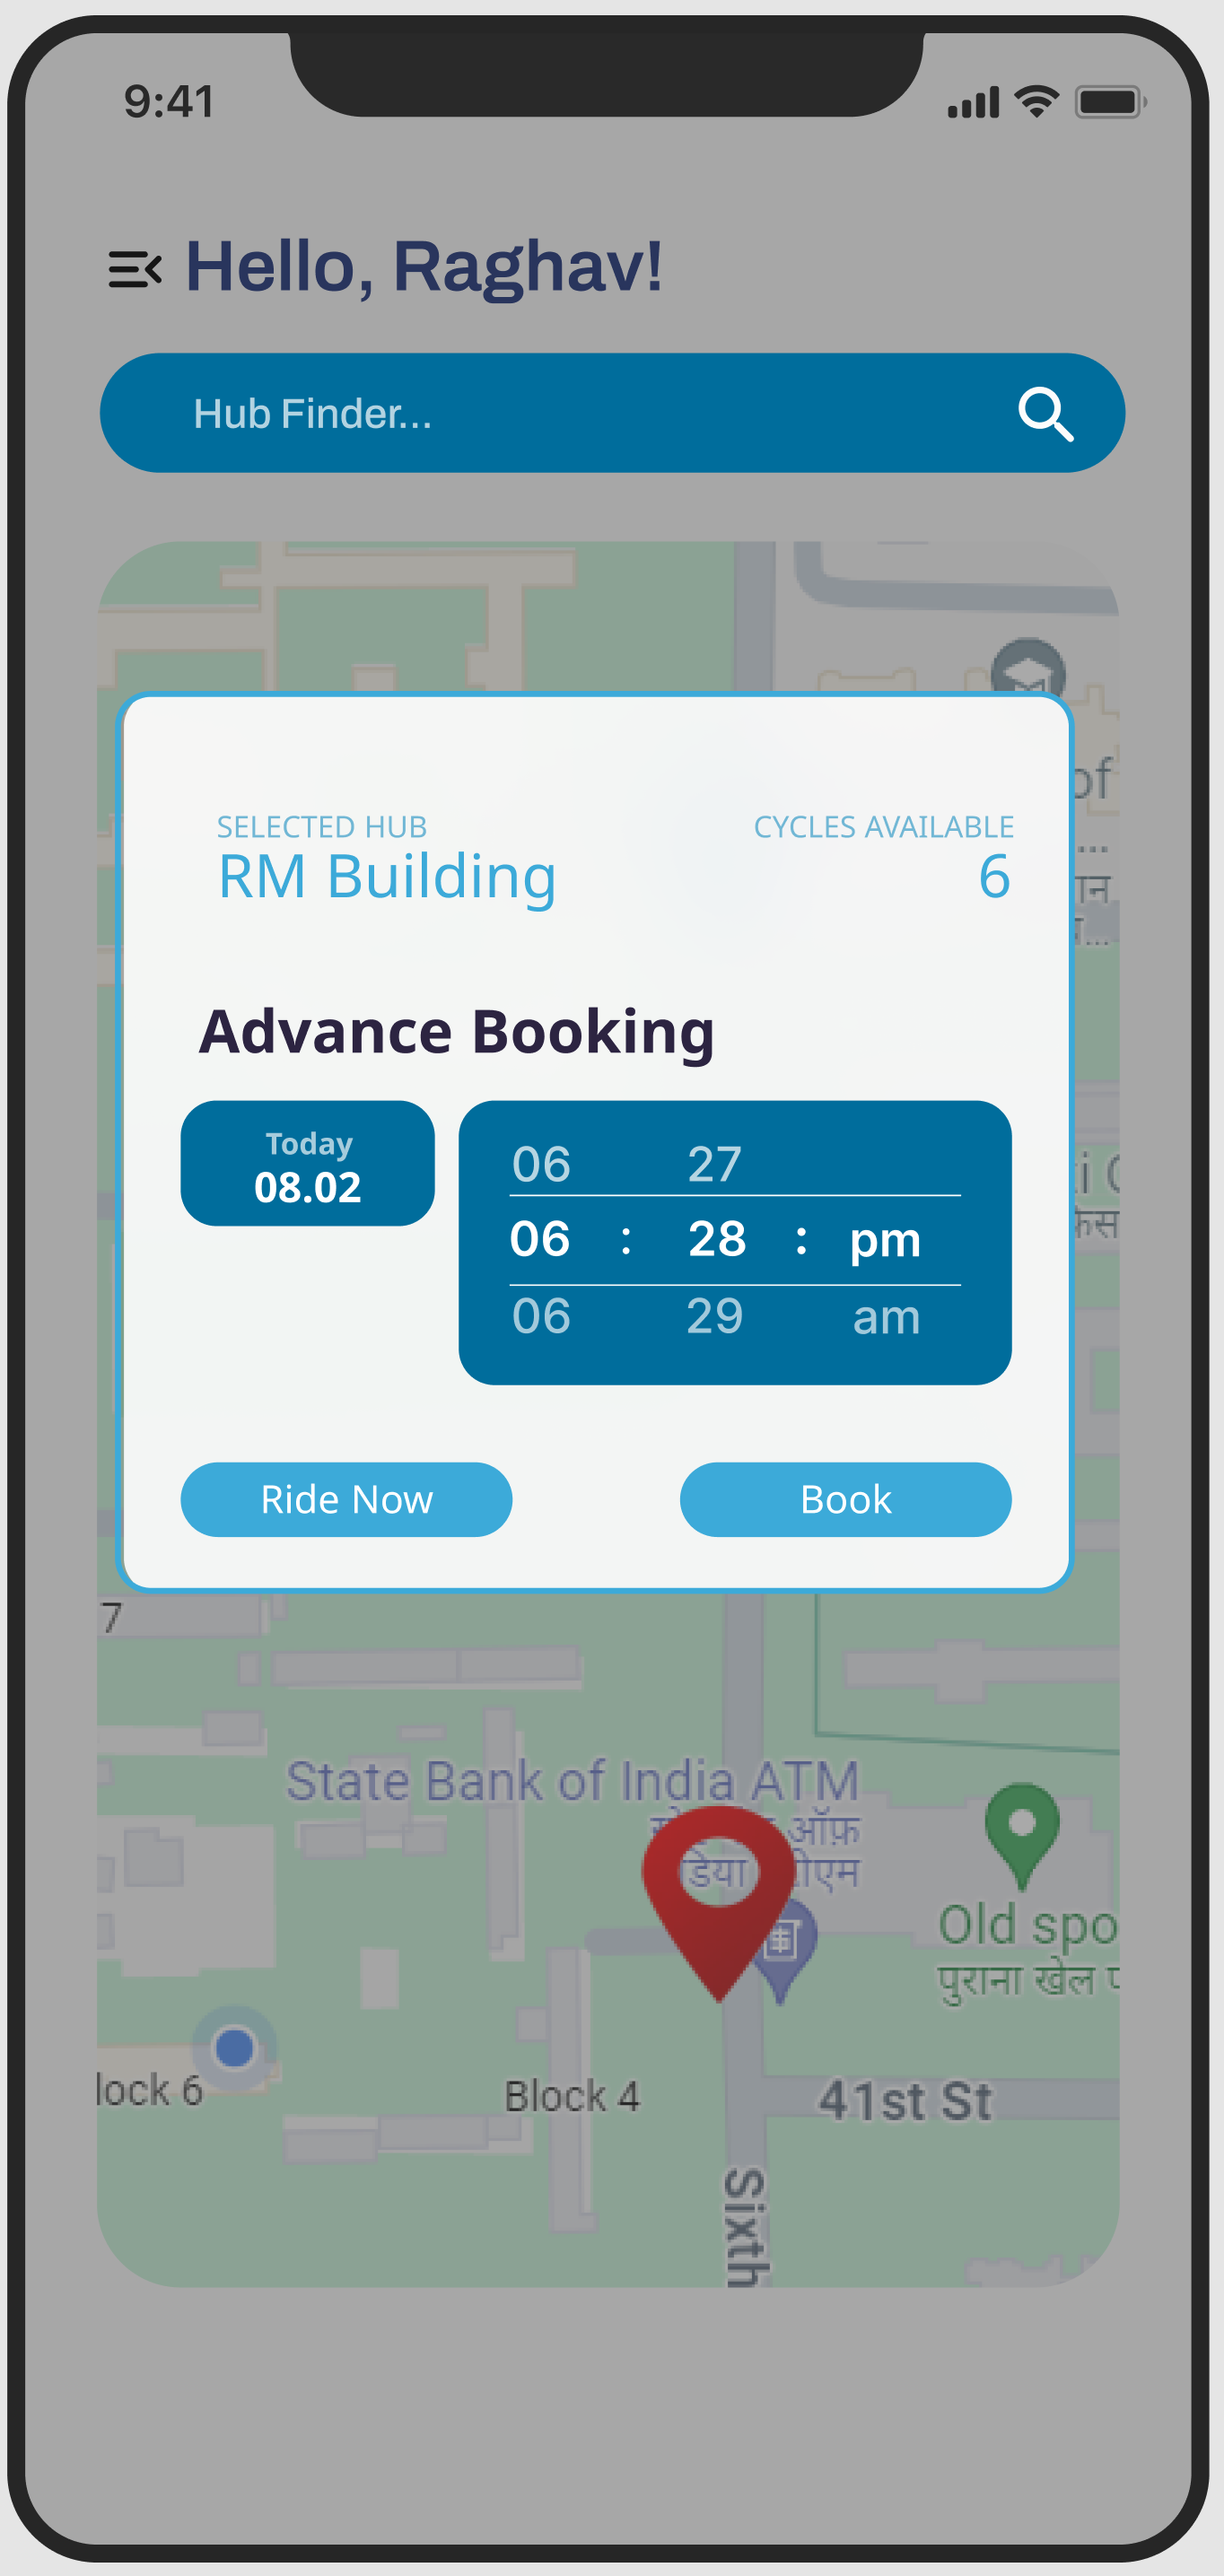
\includegraphics[scale=0.1]{ui-images/BookRideSubscribed.png}
\end{tabular}

\begin{tabular}{ccc}
    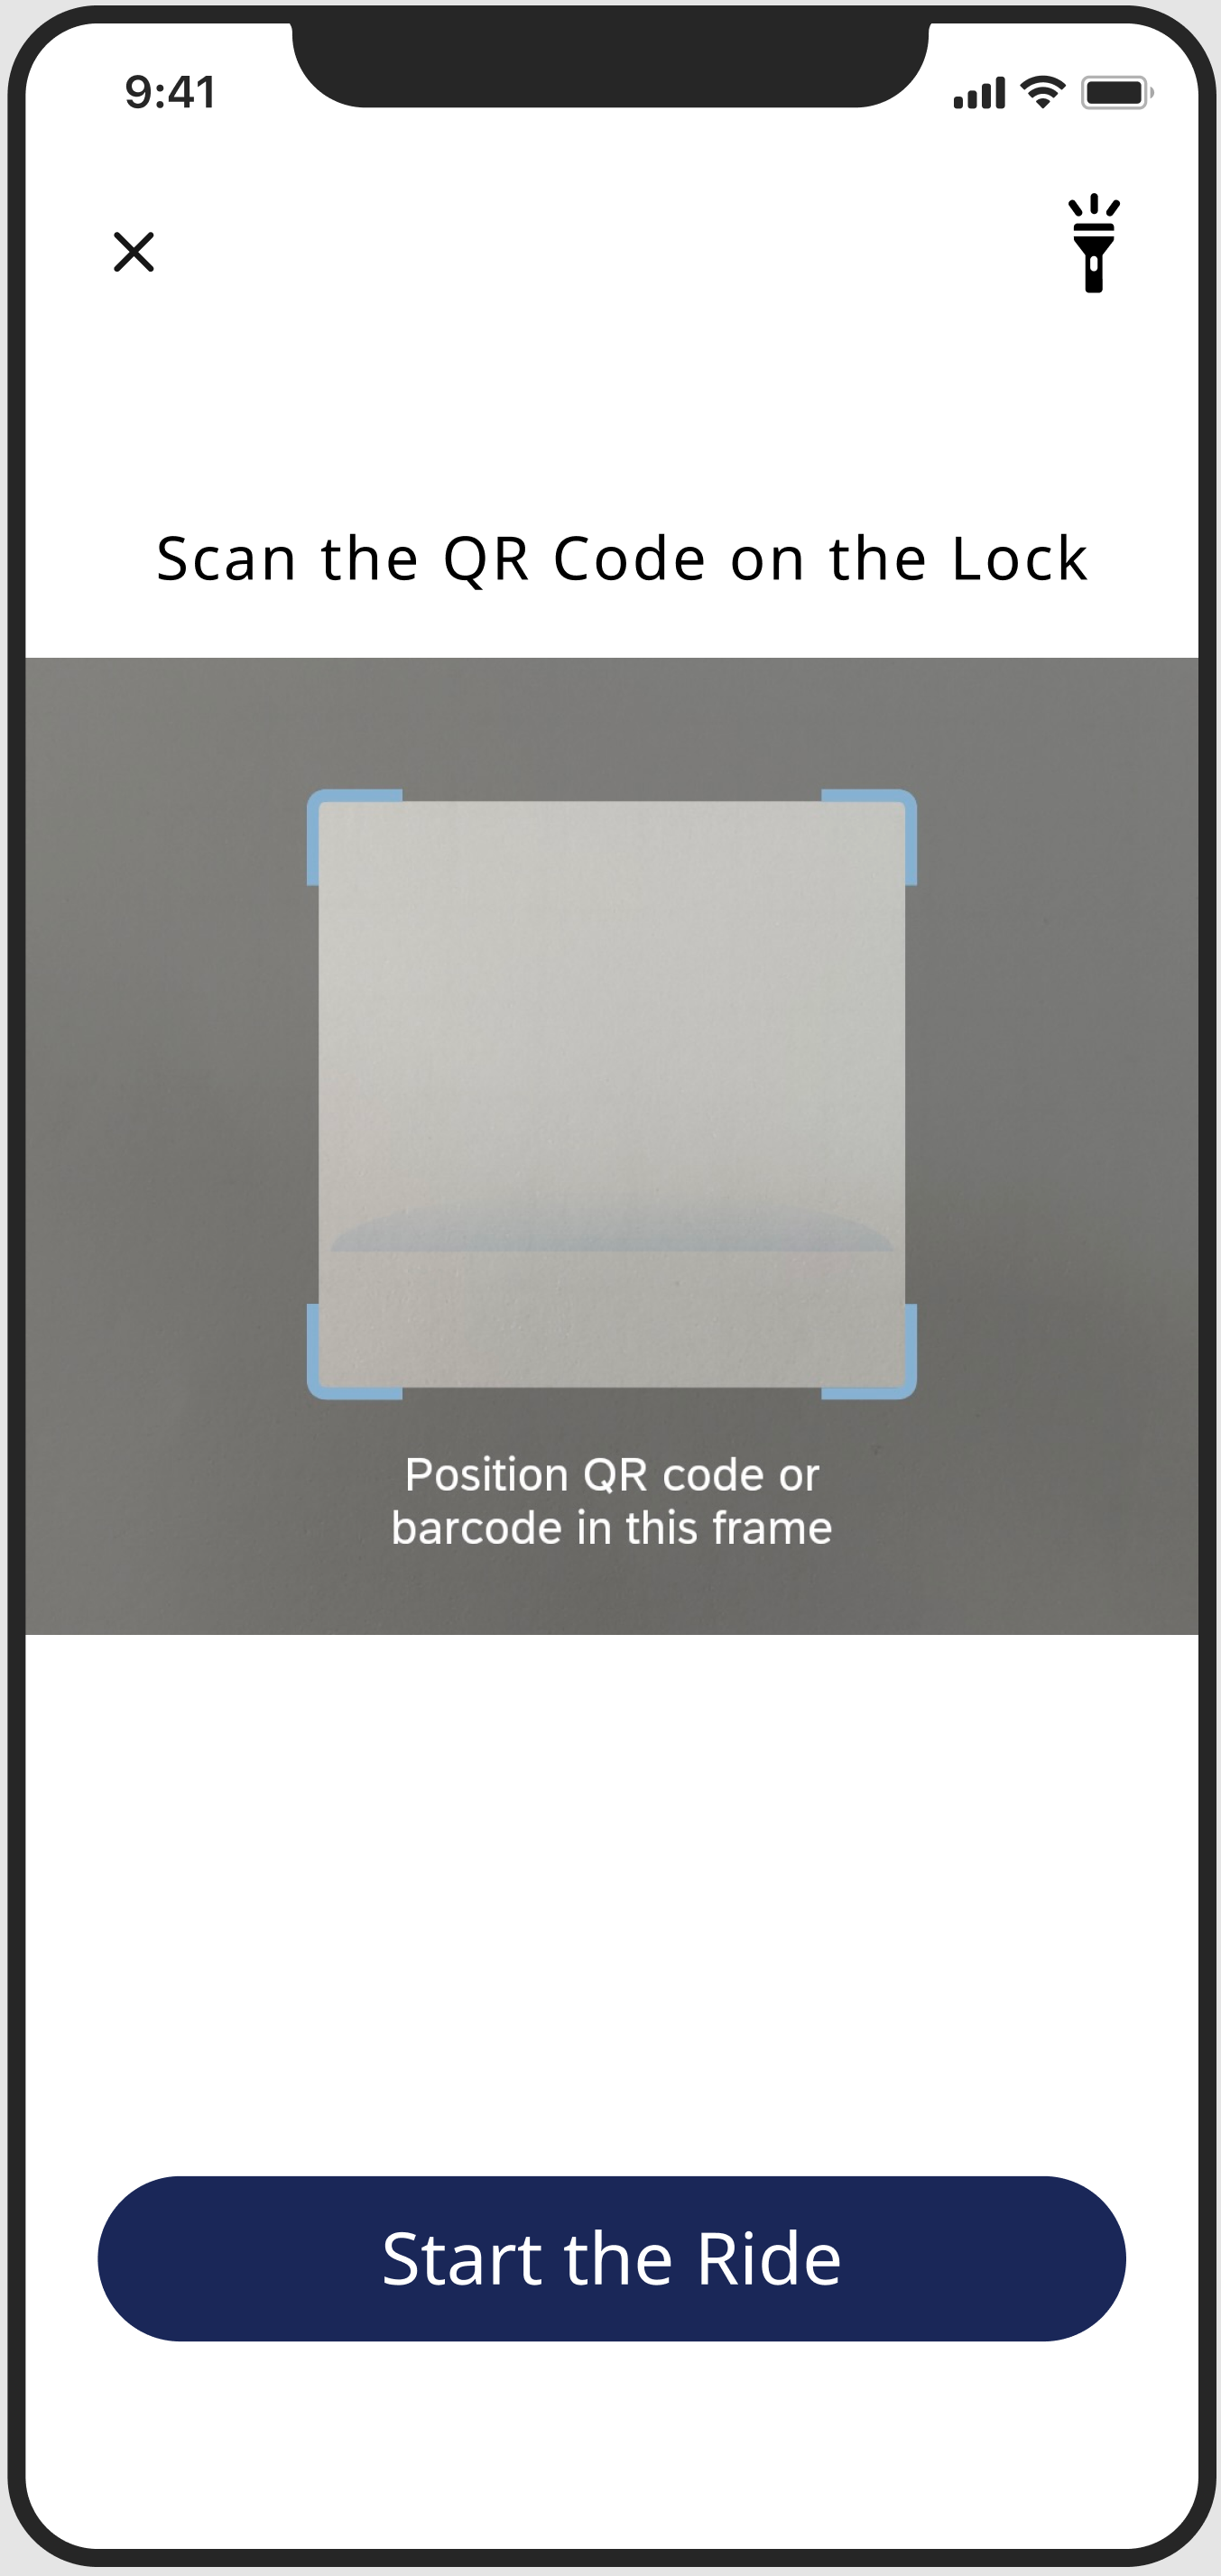
\includegraphics[scale=0.1]{ui-images/QR.png} & 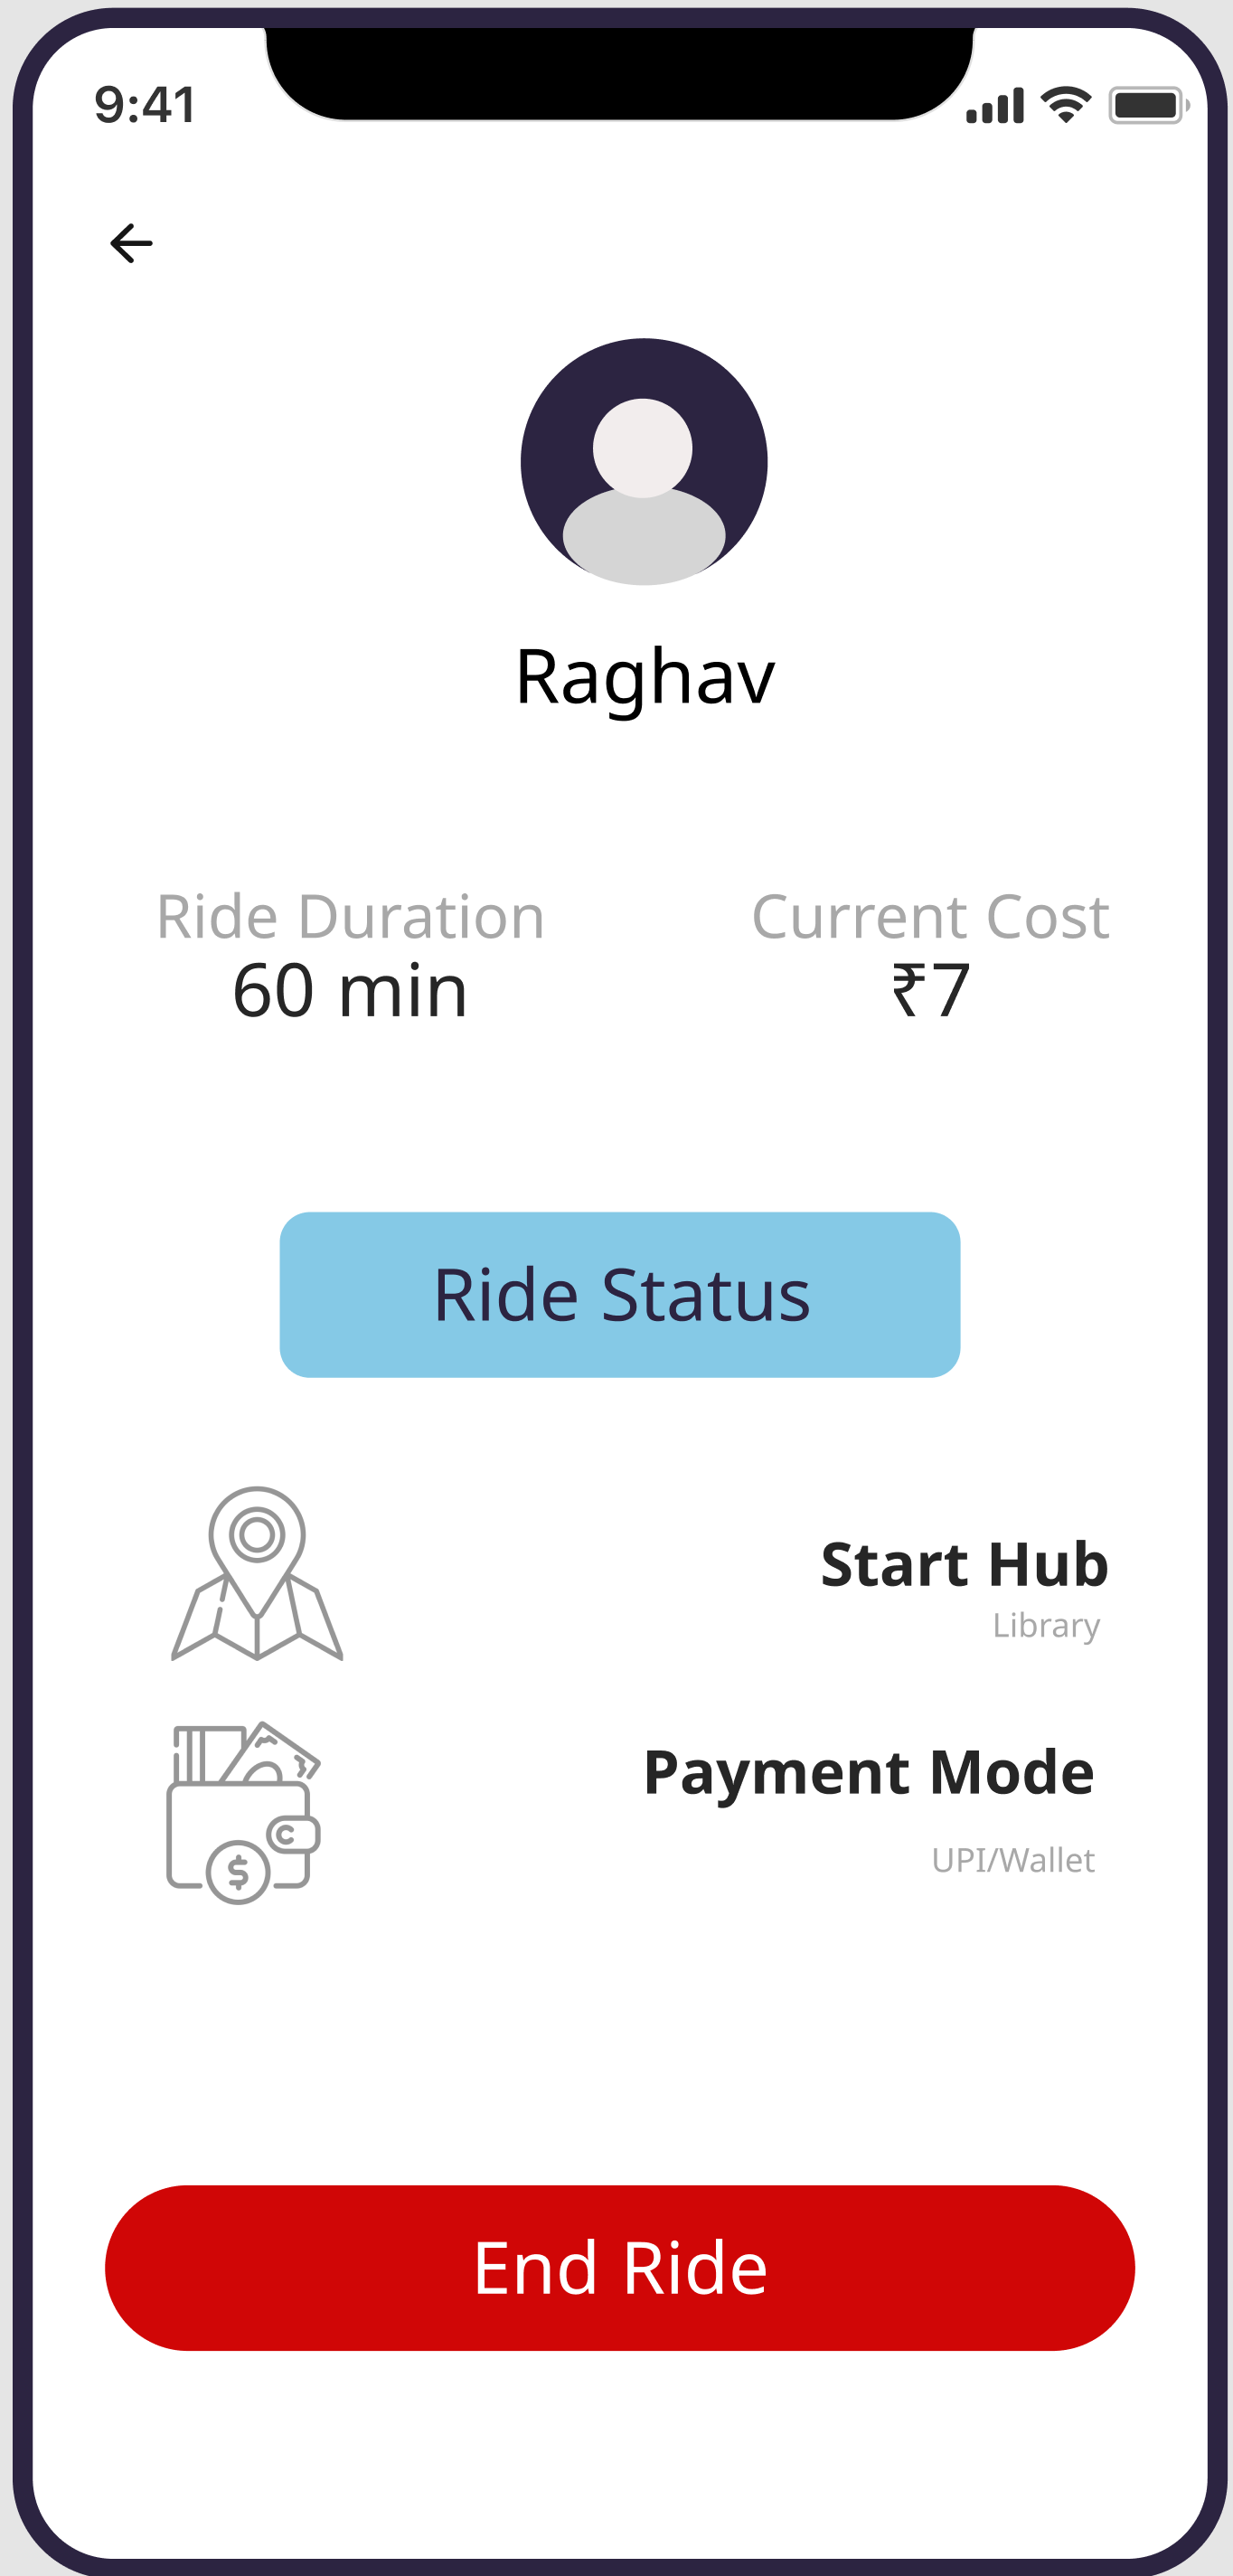
\includegraphics[scale=0.1]{ui-images/ActiveRide.png} & 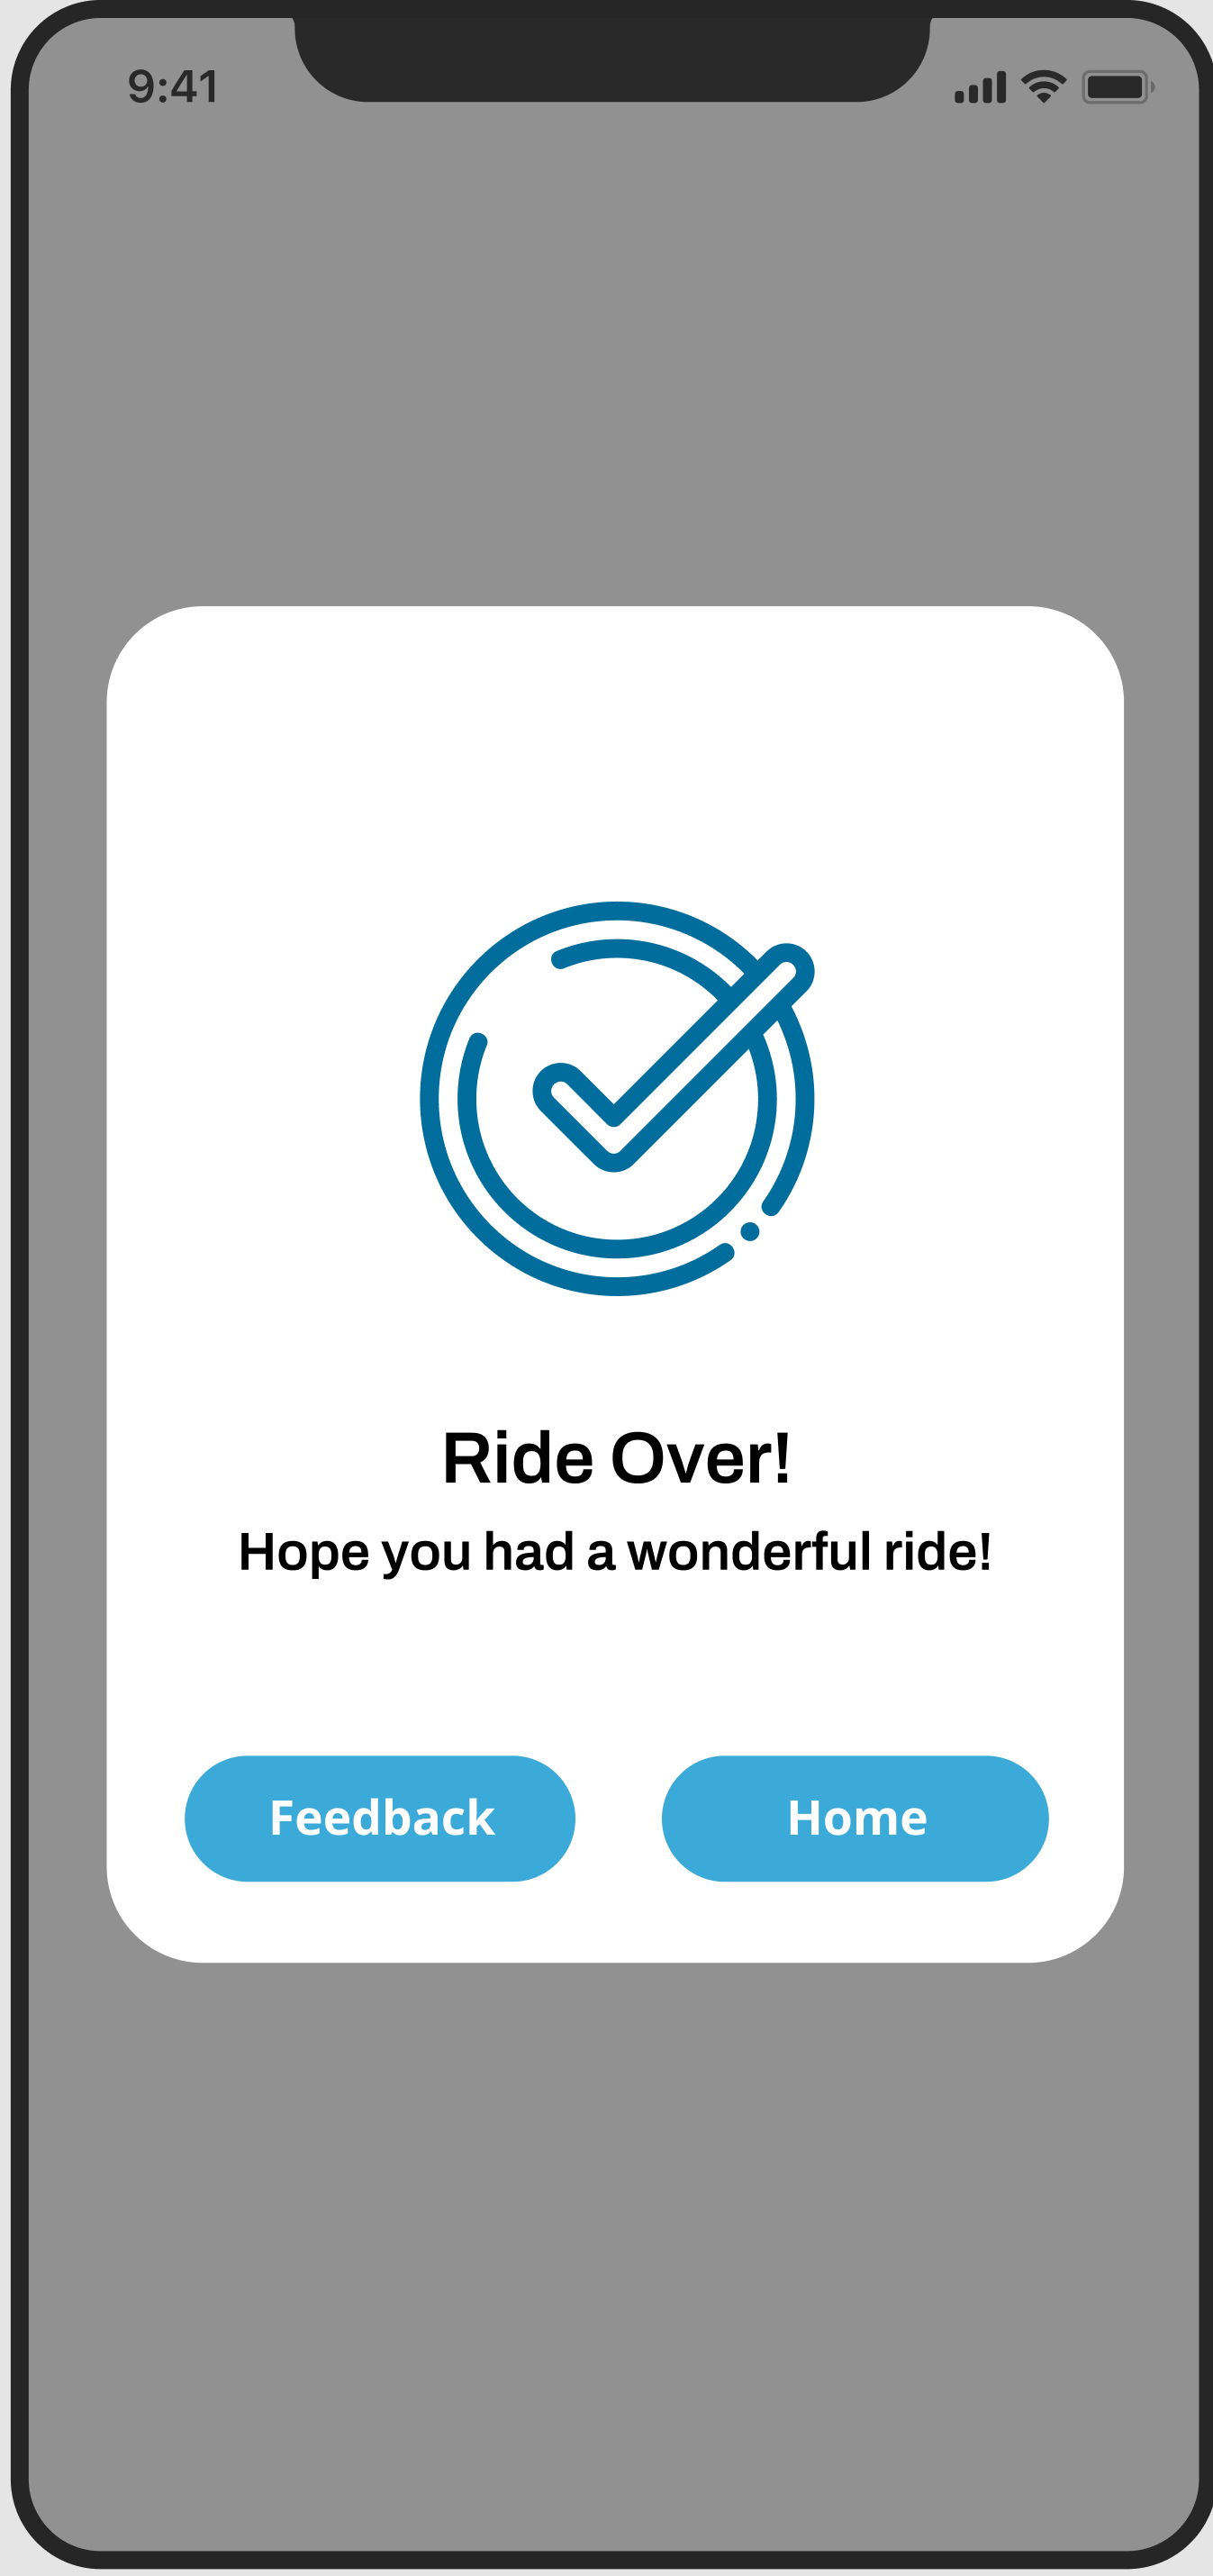
\includegraphics[scale=0.1]{ui-images/RideOver.png}
\end{tabular}
\end{center}

\subsubsection{User Feedback}
The user can select any issue they faced during the ride and provide a description. The user can also provide feedback on the ride.
\begin{center}
\begin{tabular}{ccc}
    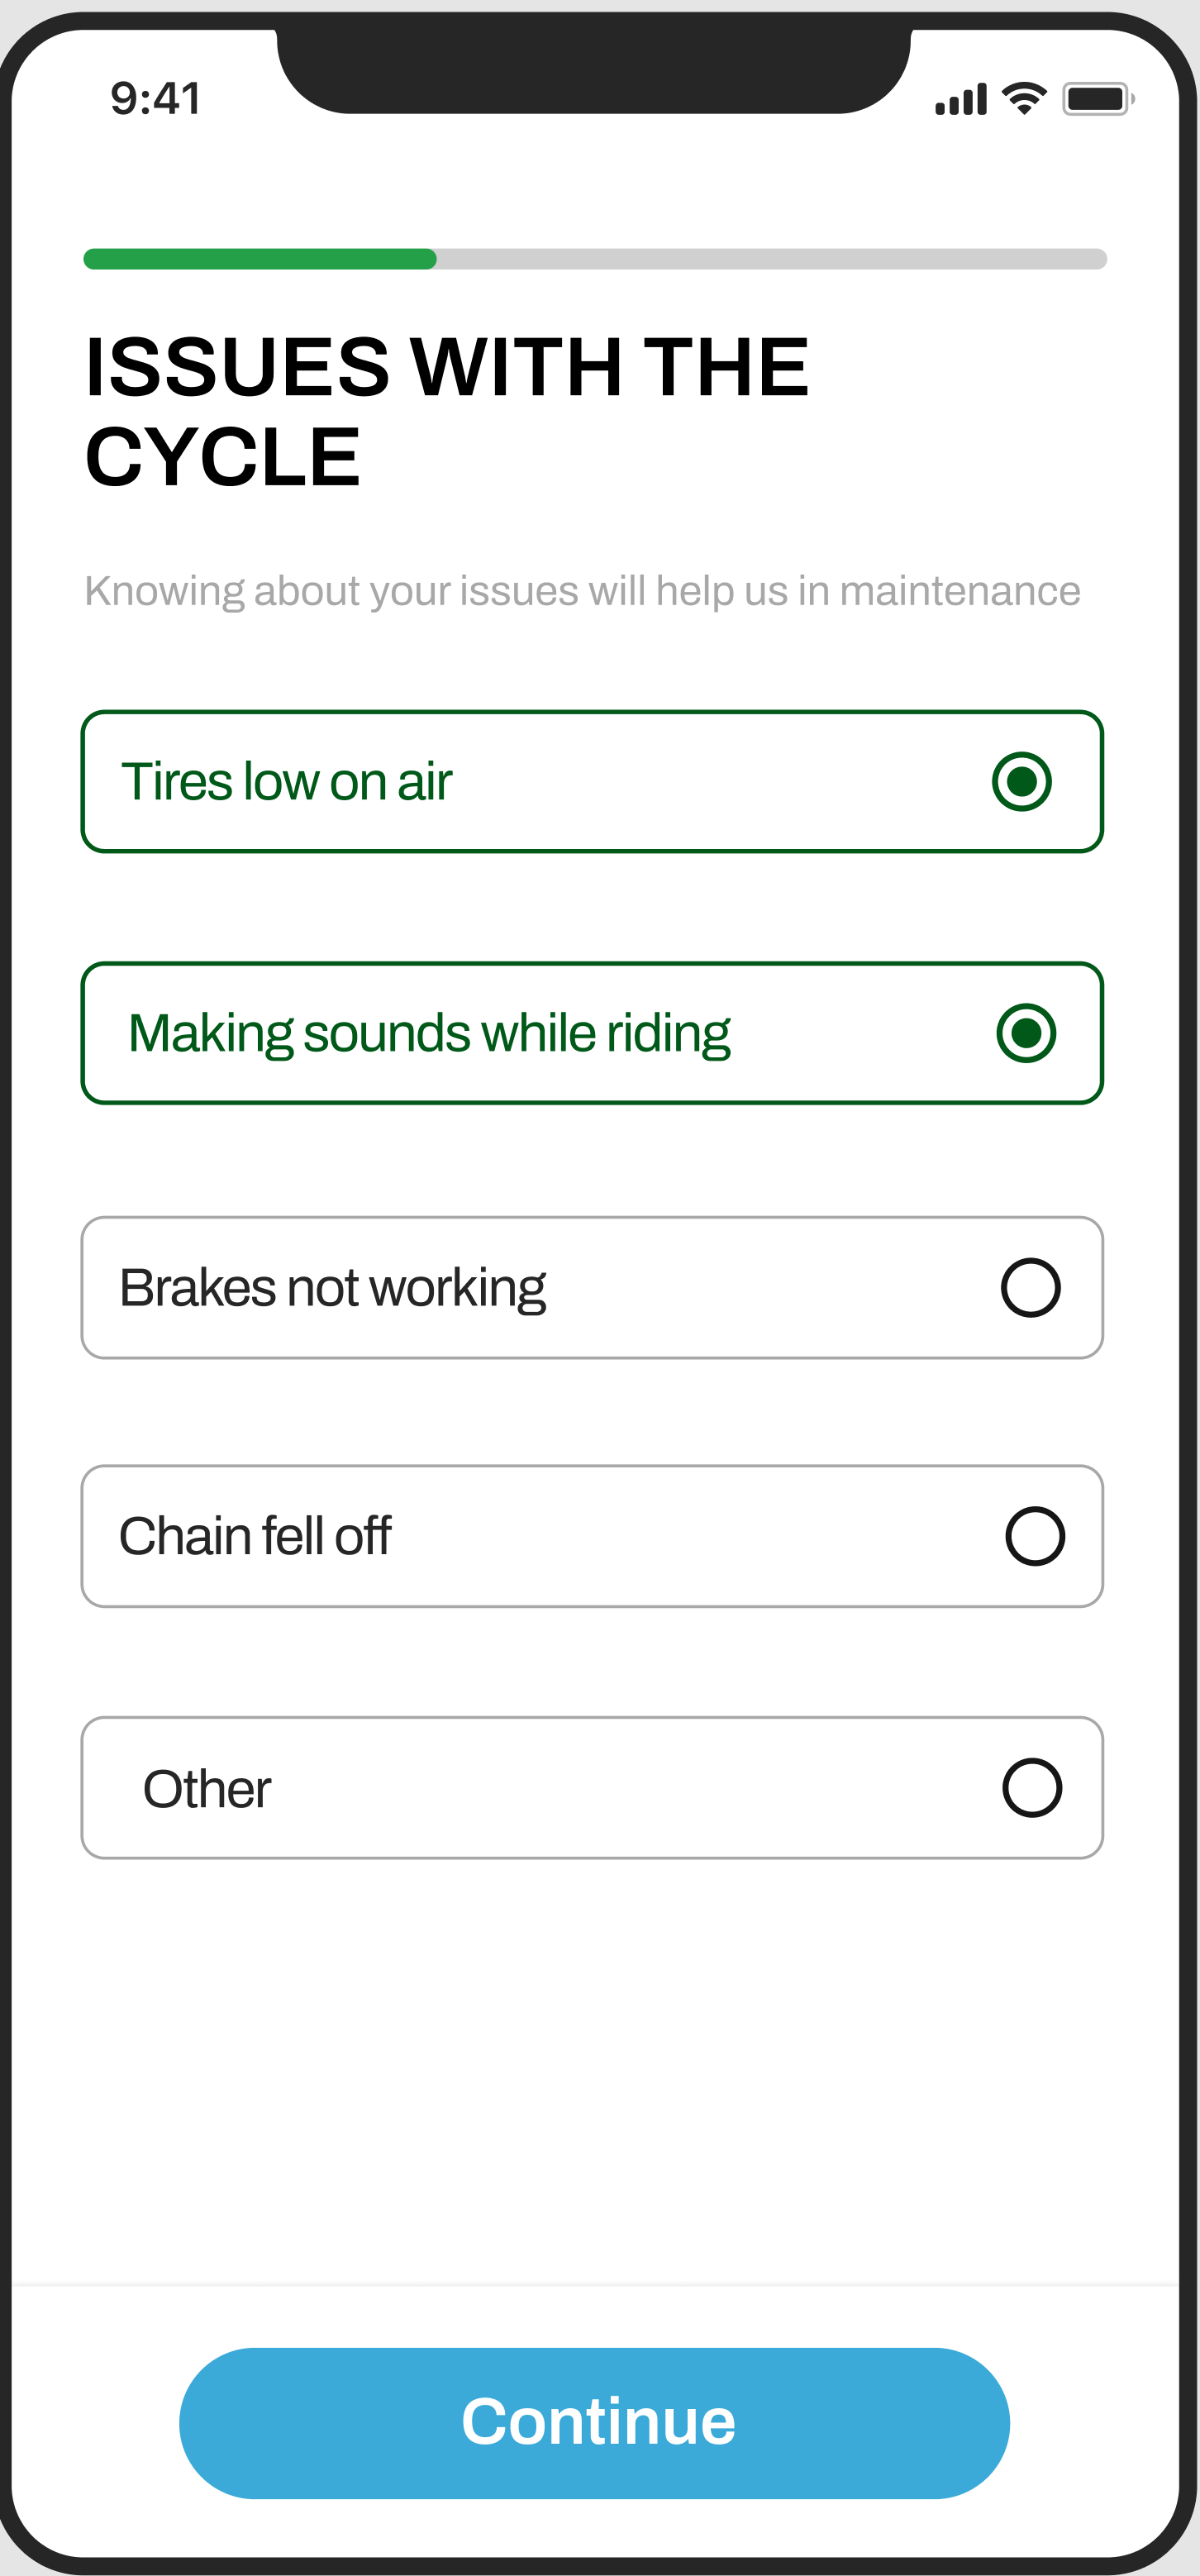
\includegraphics[scale=0.1]{ui-images/CycleIssues.png} & 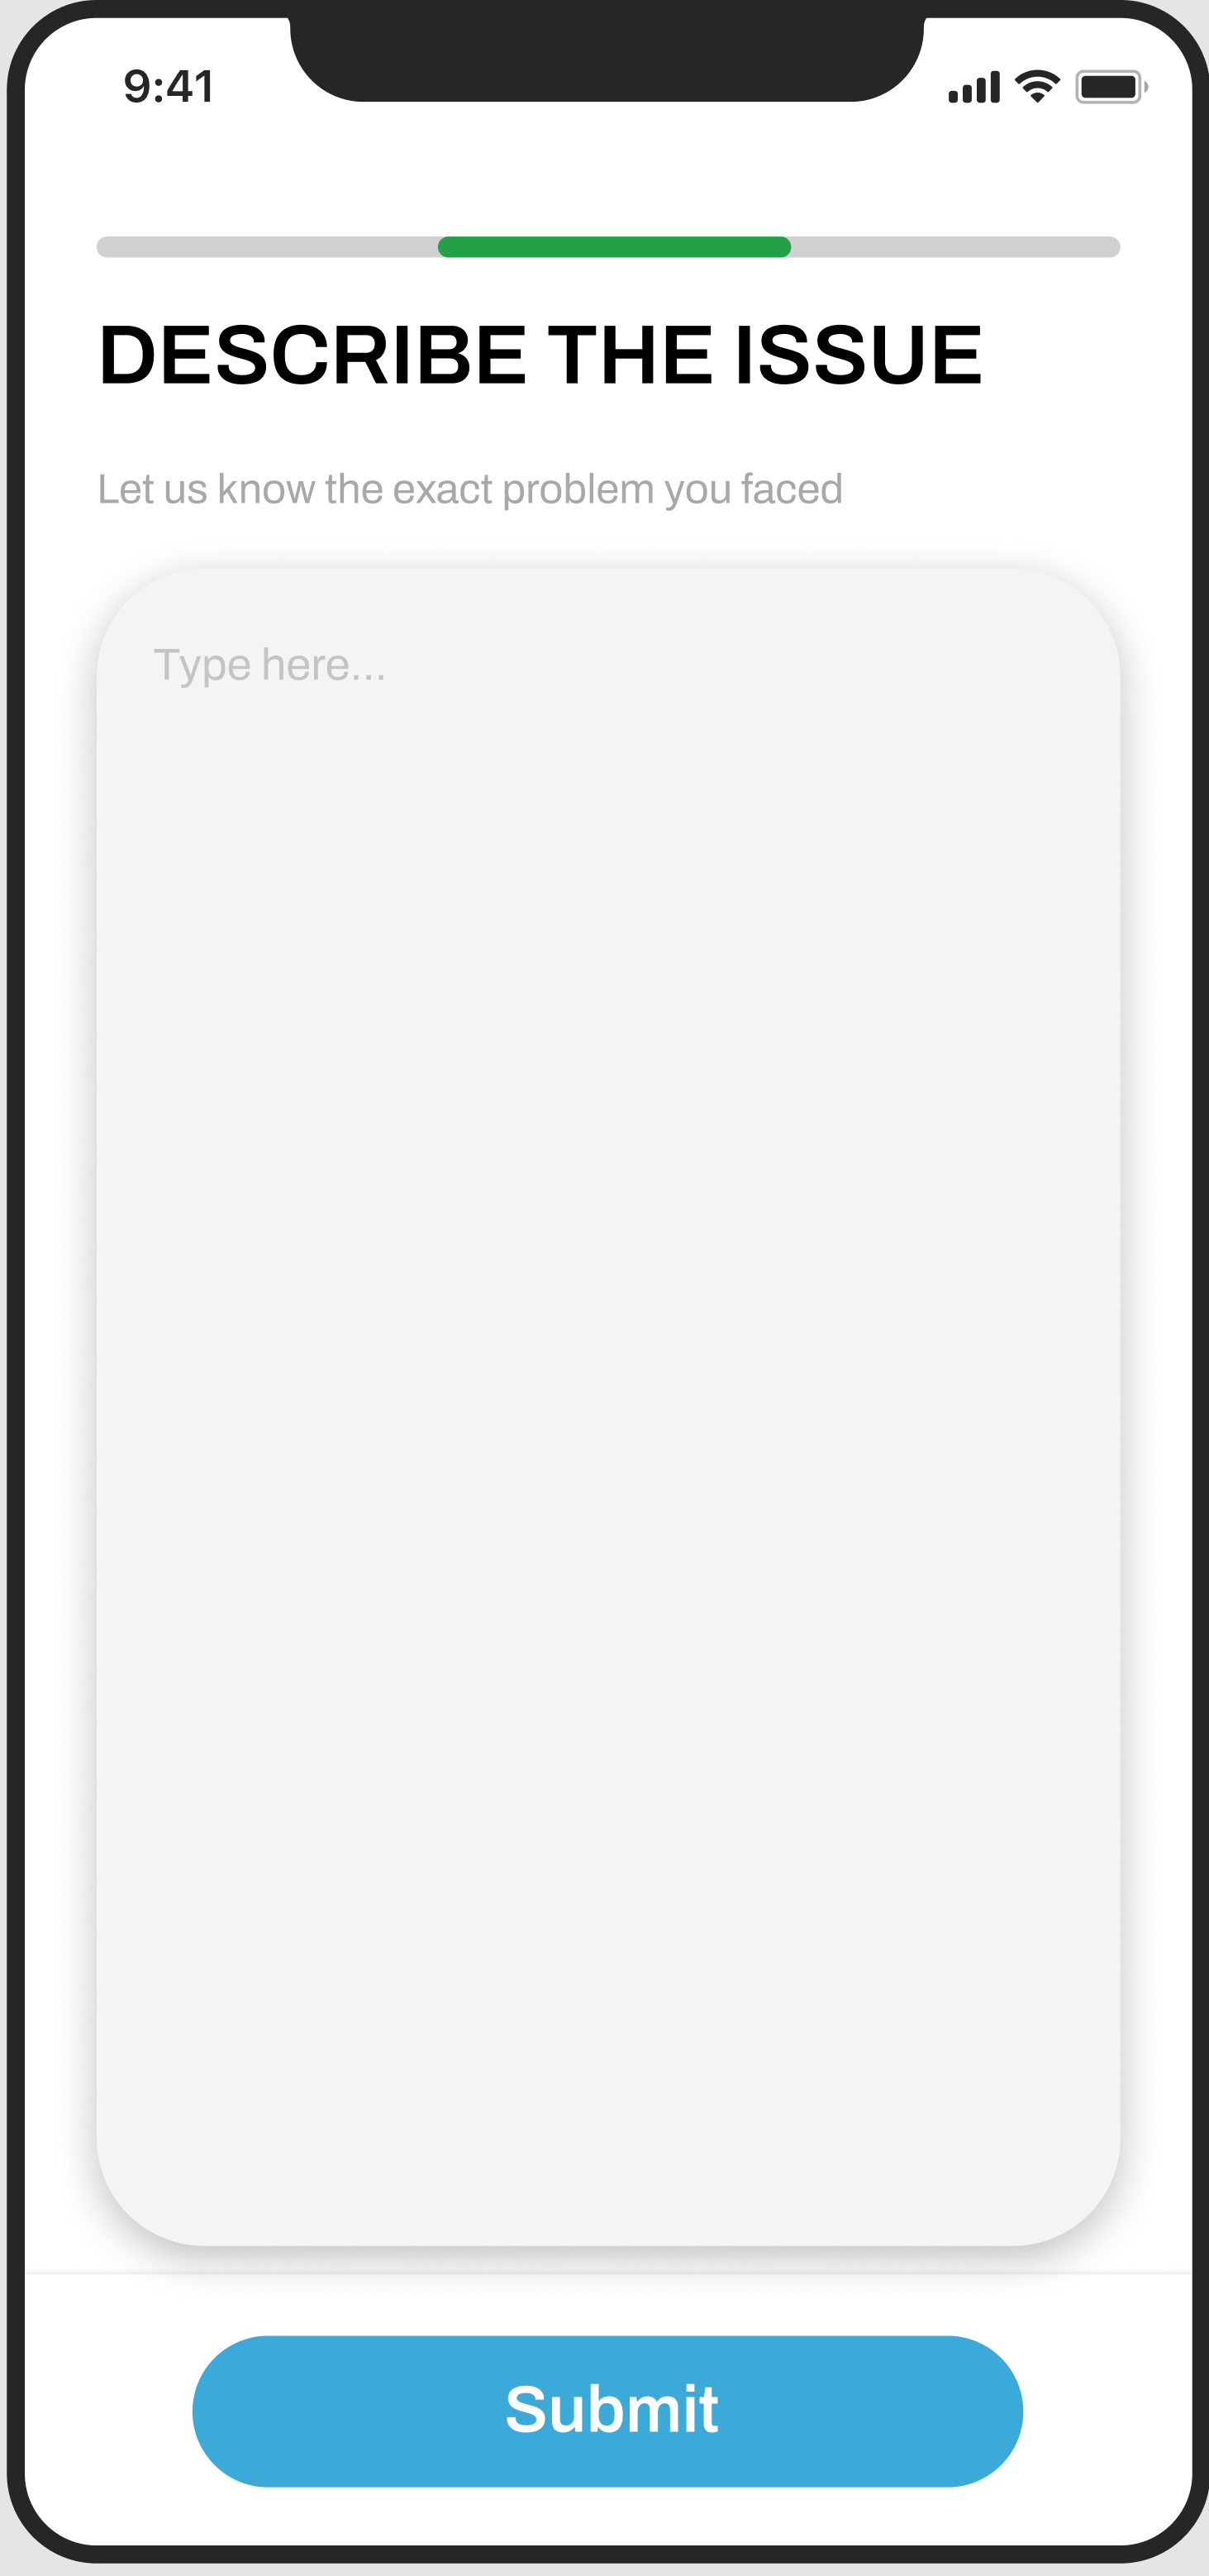
\includegraphics[scale=0.1]{ui-images/IssueDescription.png} & 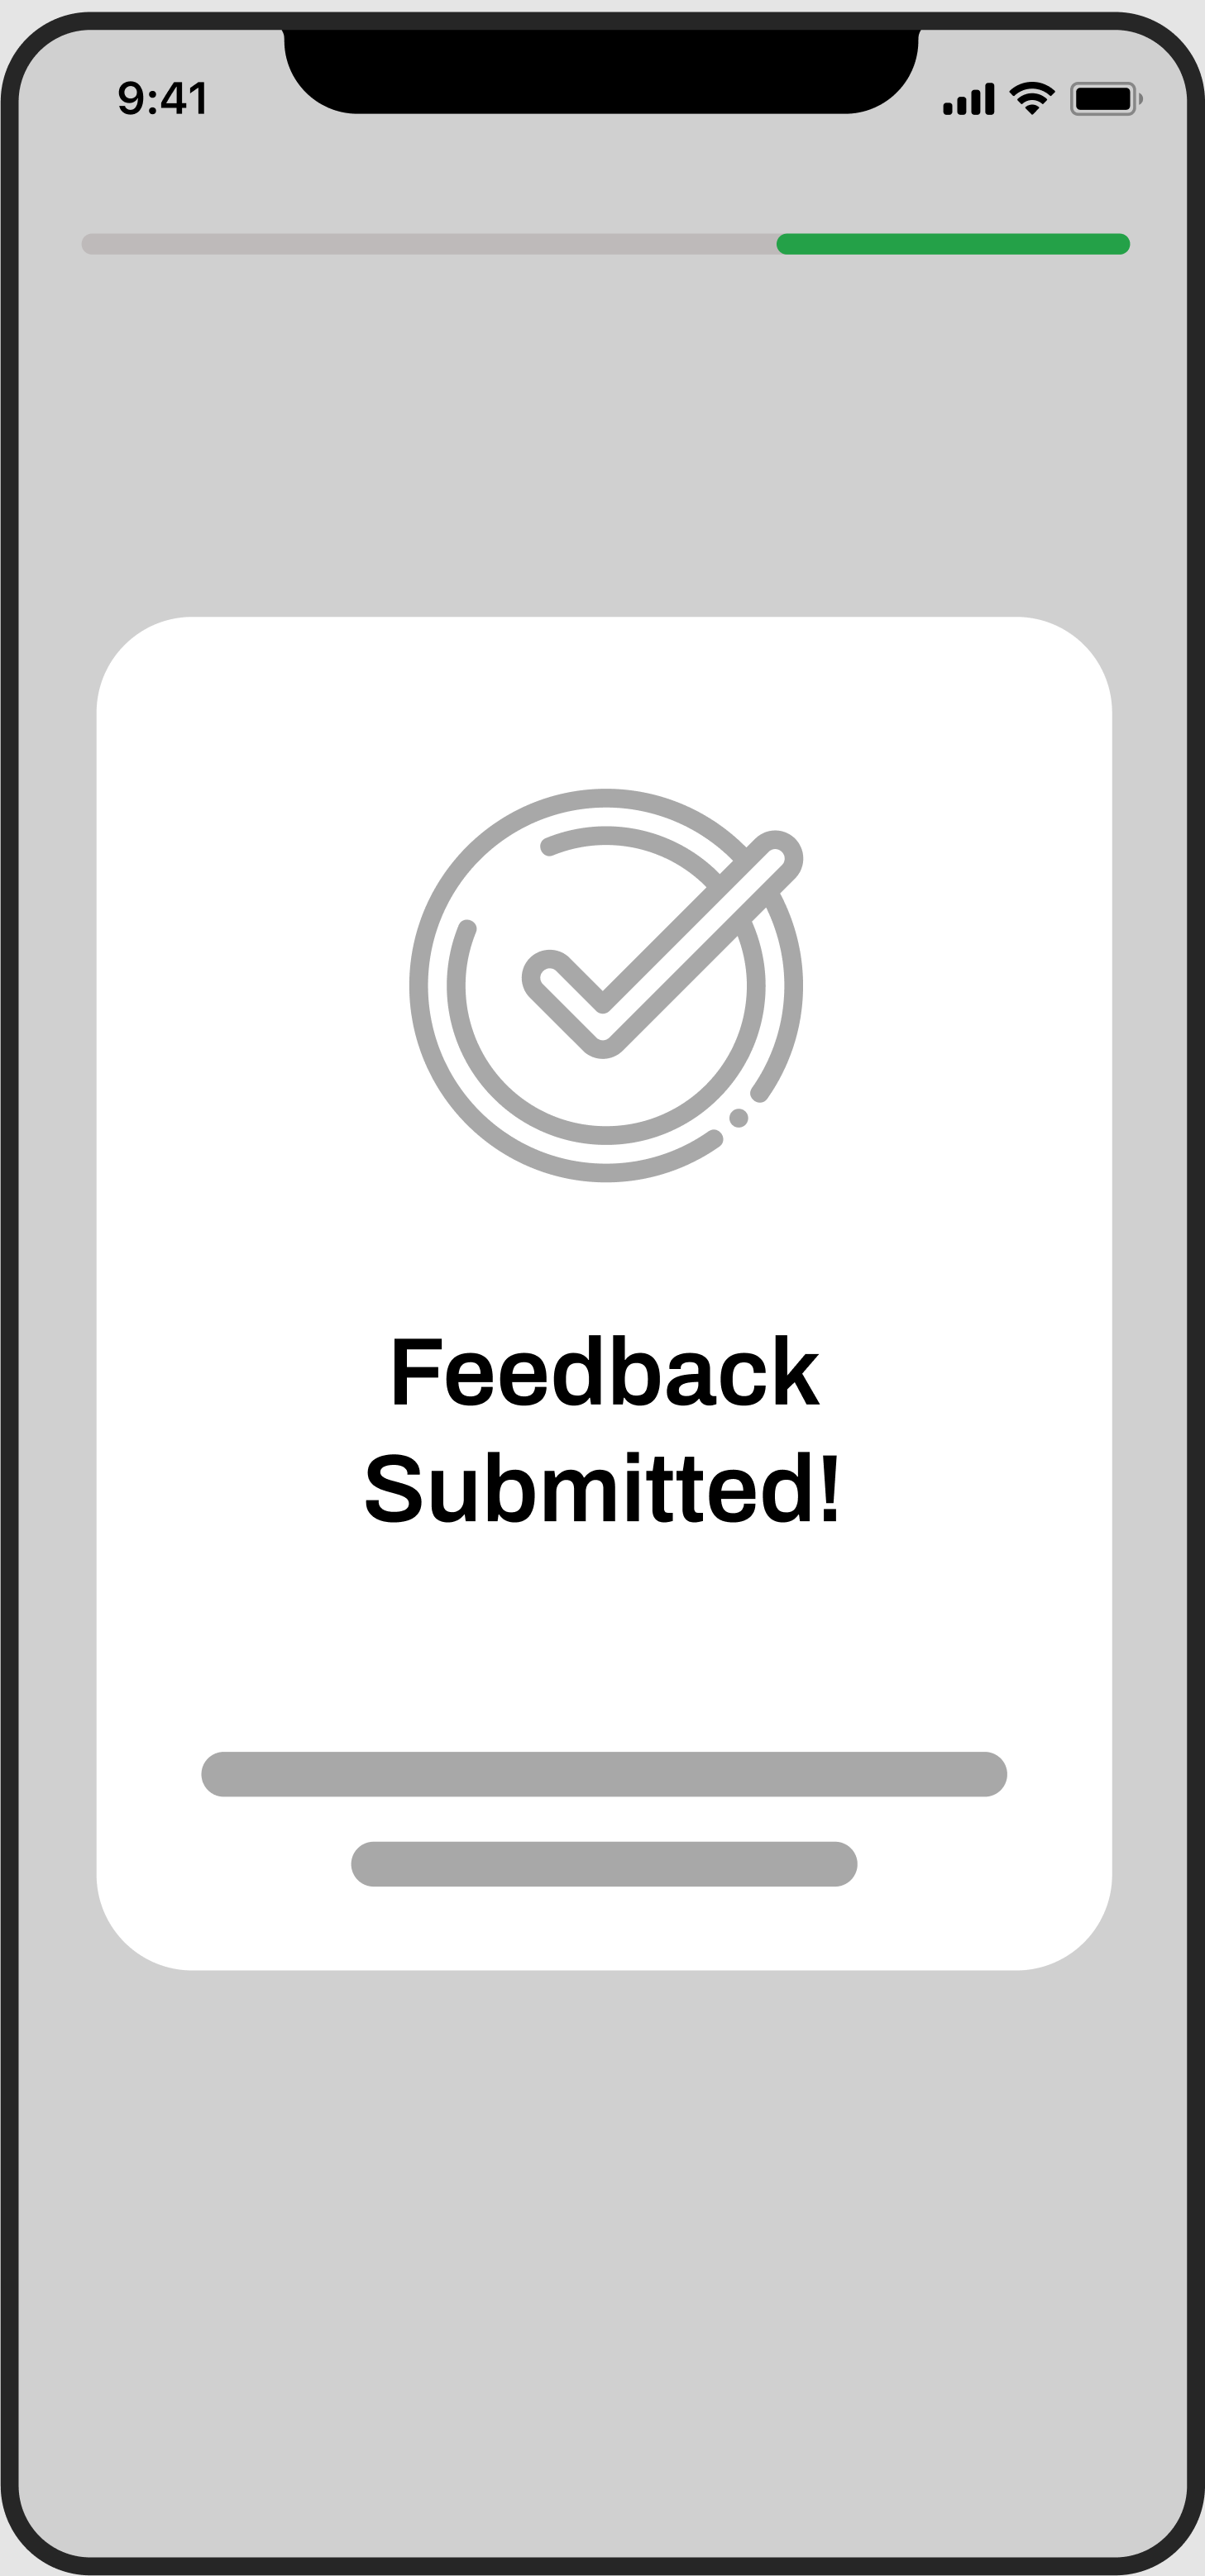
\includegraphics[scale=0.1]{ui-images/FeedbackSubmission.png}
\end{tabular}
\end{center}

\subsubsection{Subscription Model}
The option of booking rides in advance is only available for subscribed users. This option is greyed out in case the user is not subscribed. If they tap on any greyed out option, an advertisement for the subscription model is shown.
\begin{center}
    \begin{tabular}{cc}
        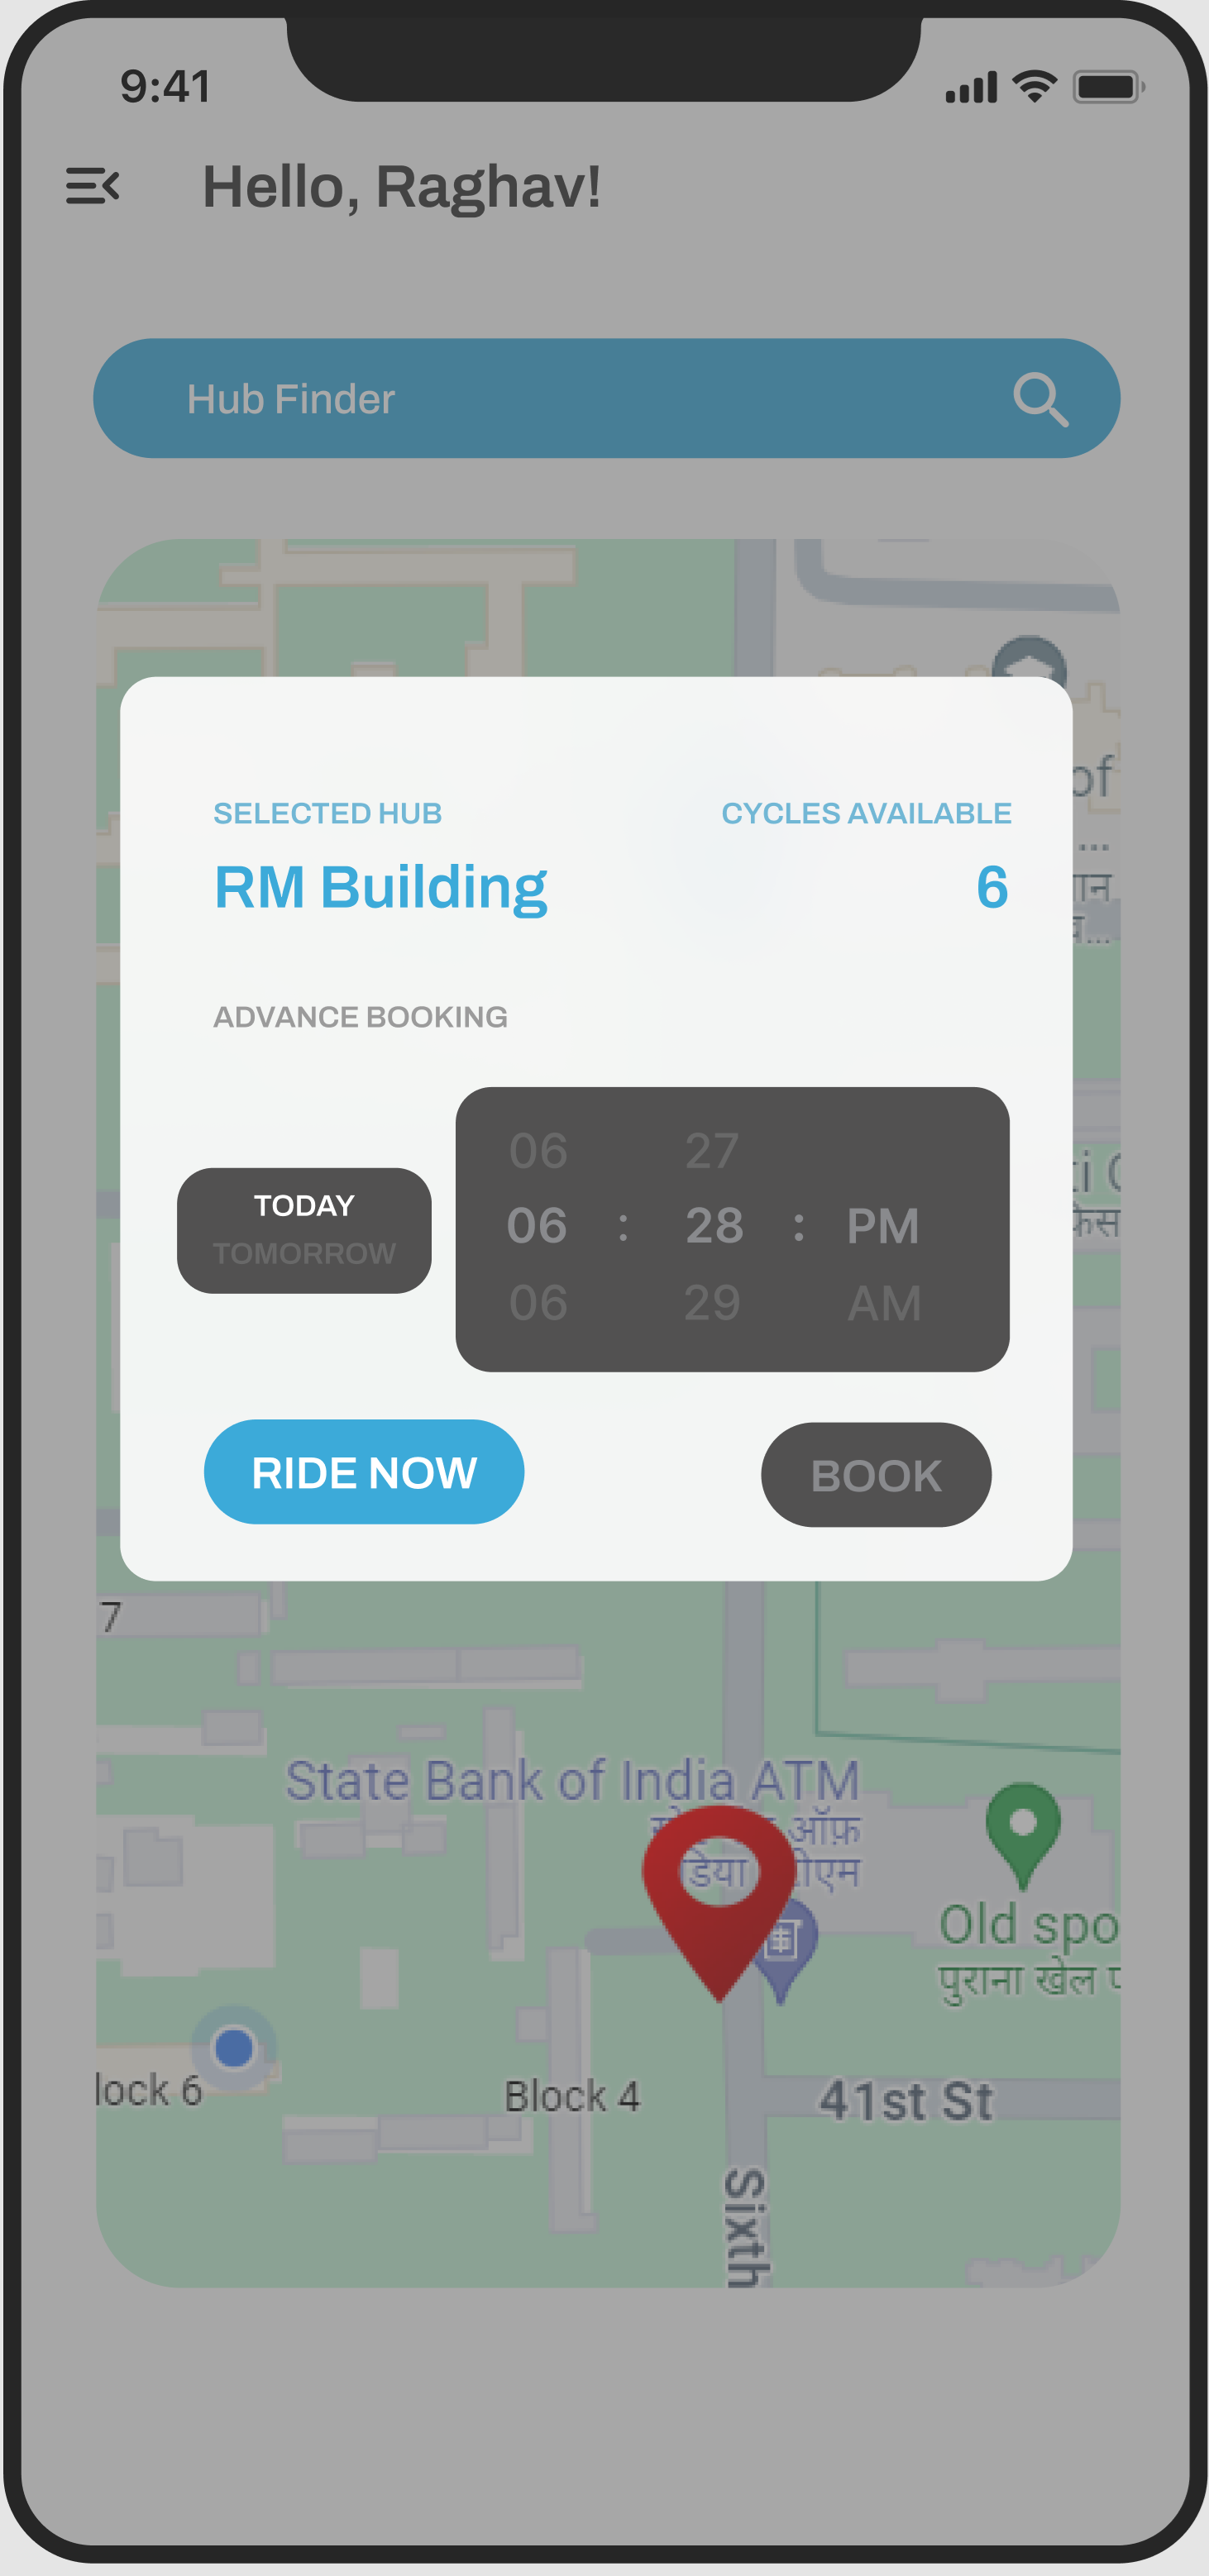
\includegraphics[scale=0.1]{ui-images/BookRideUnsubscribed.png} & 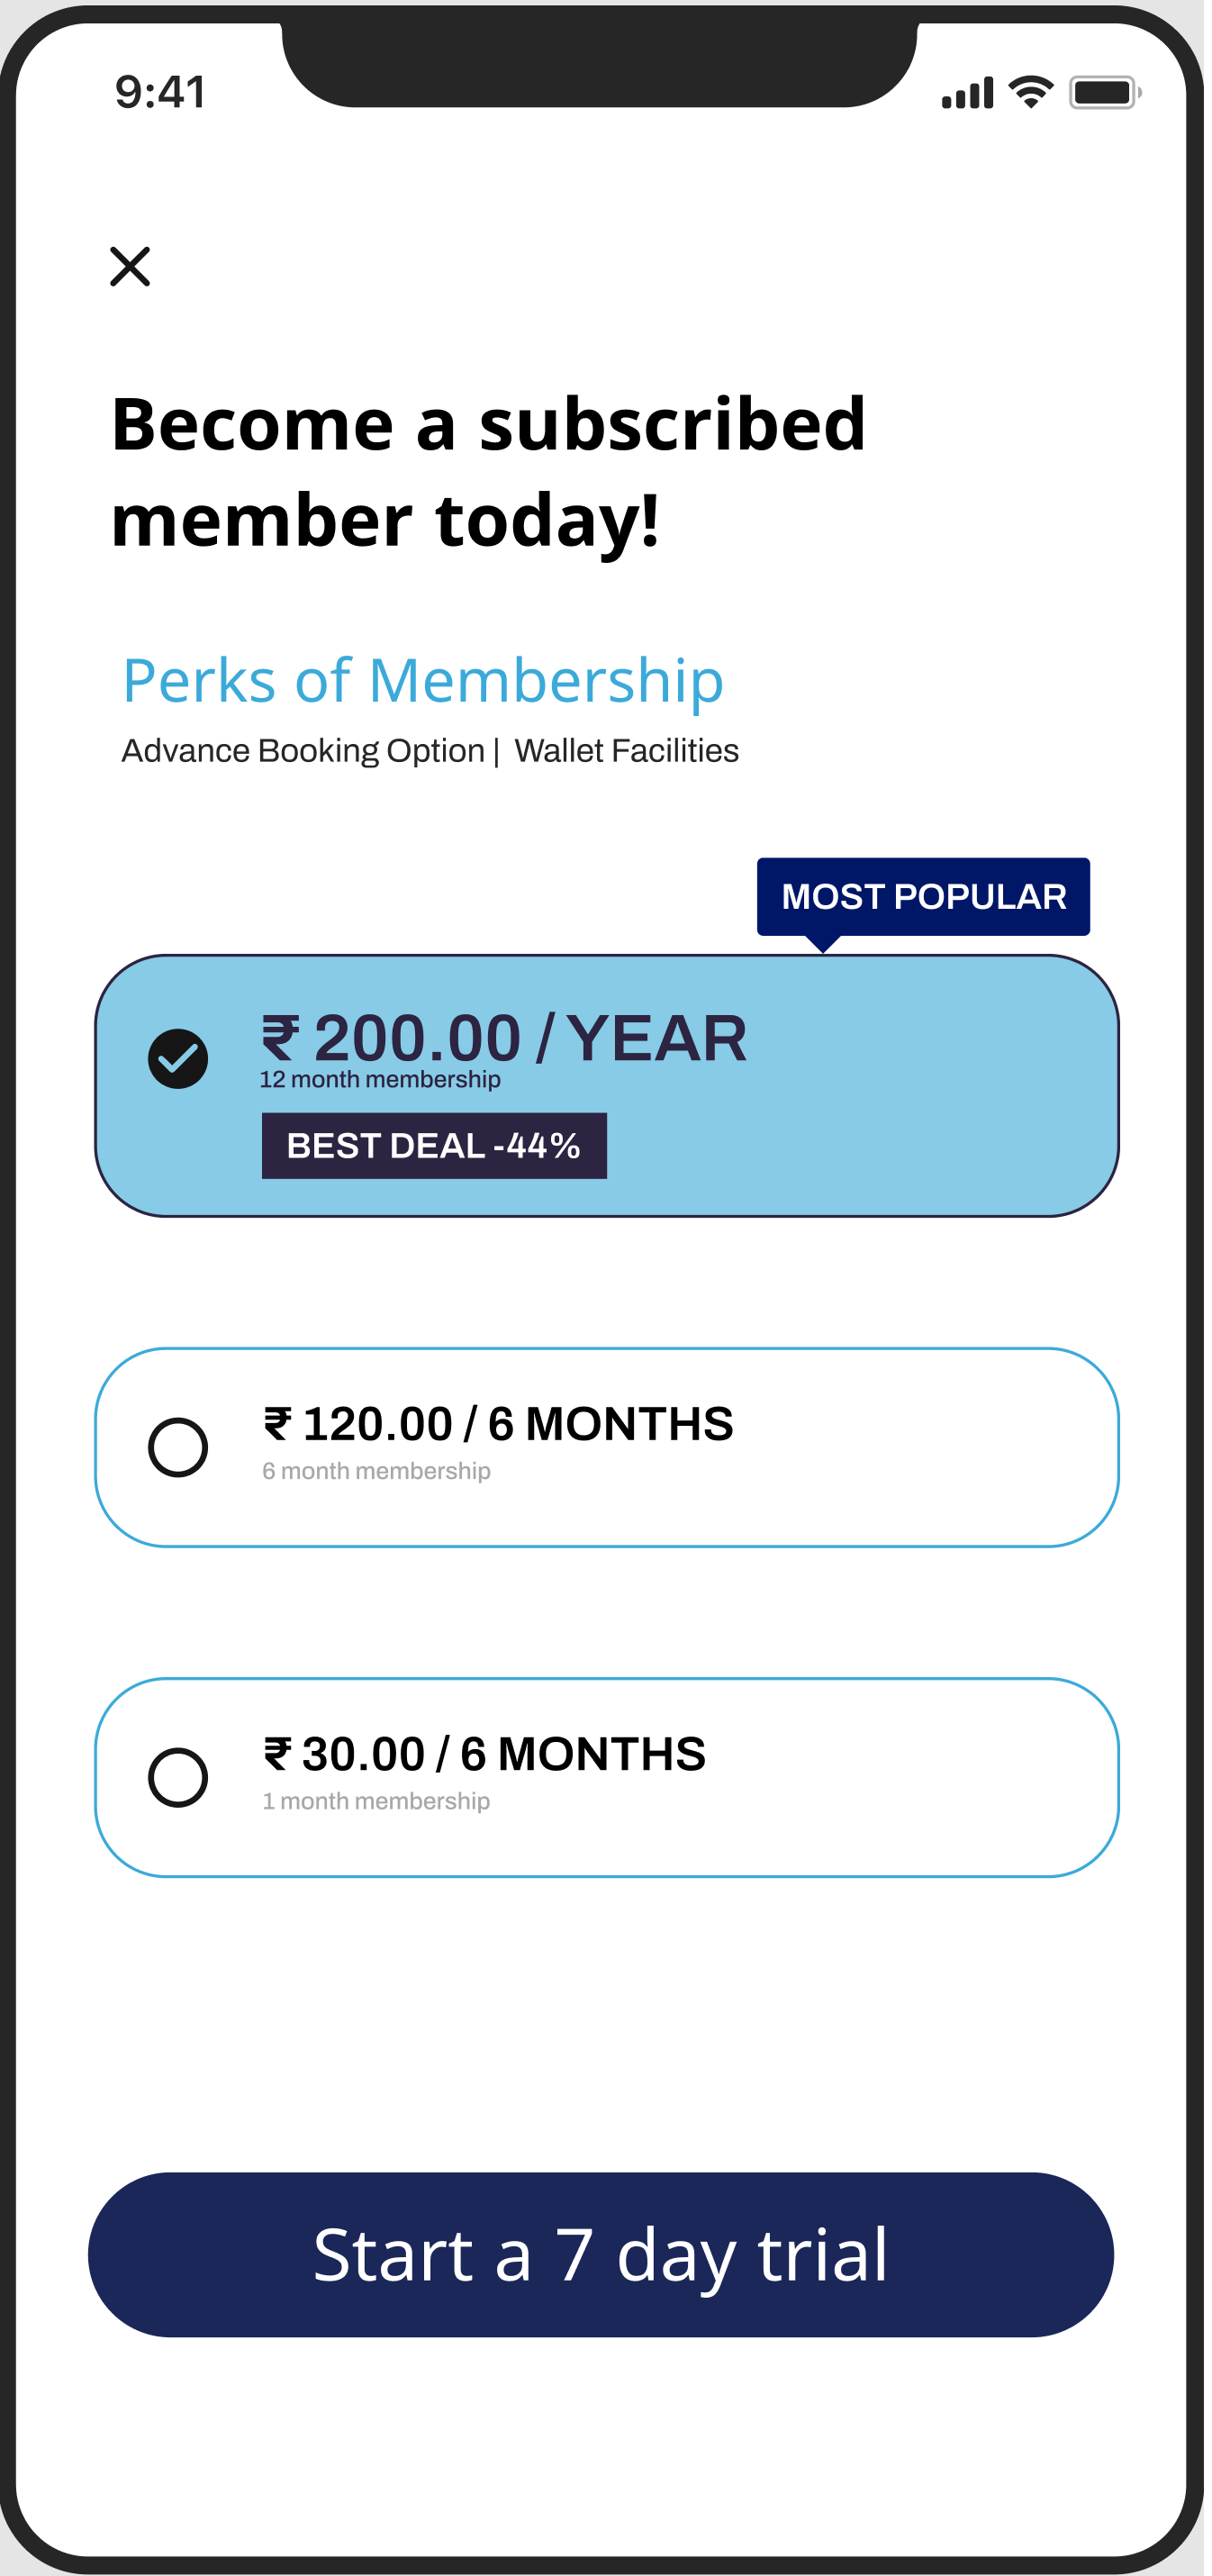
\includegraphics[scale=0.1]{ui-images/Advertisement.png}
    \end{tabular}
\end{center}

\subsubsection{Settings and Analytics View}
The navigation bar presents the user with options to view their wallet details, ride history, settings, bookings, and to log out. 
\begin{center}
\begin{tabular}{ccc}
    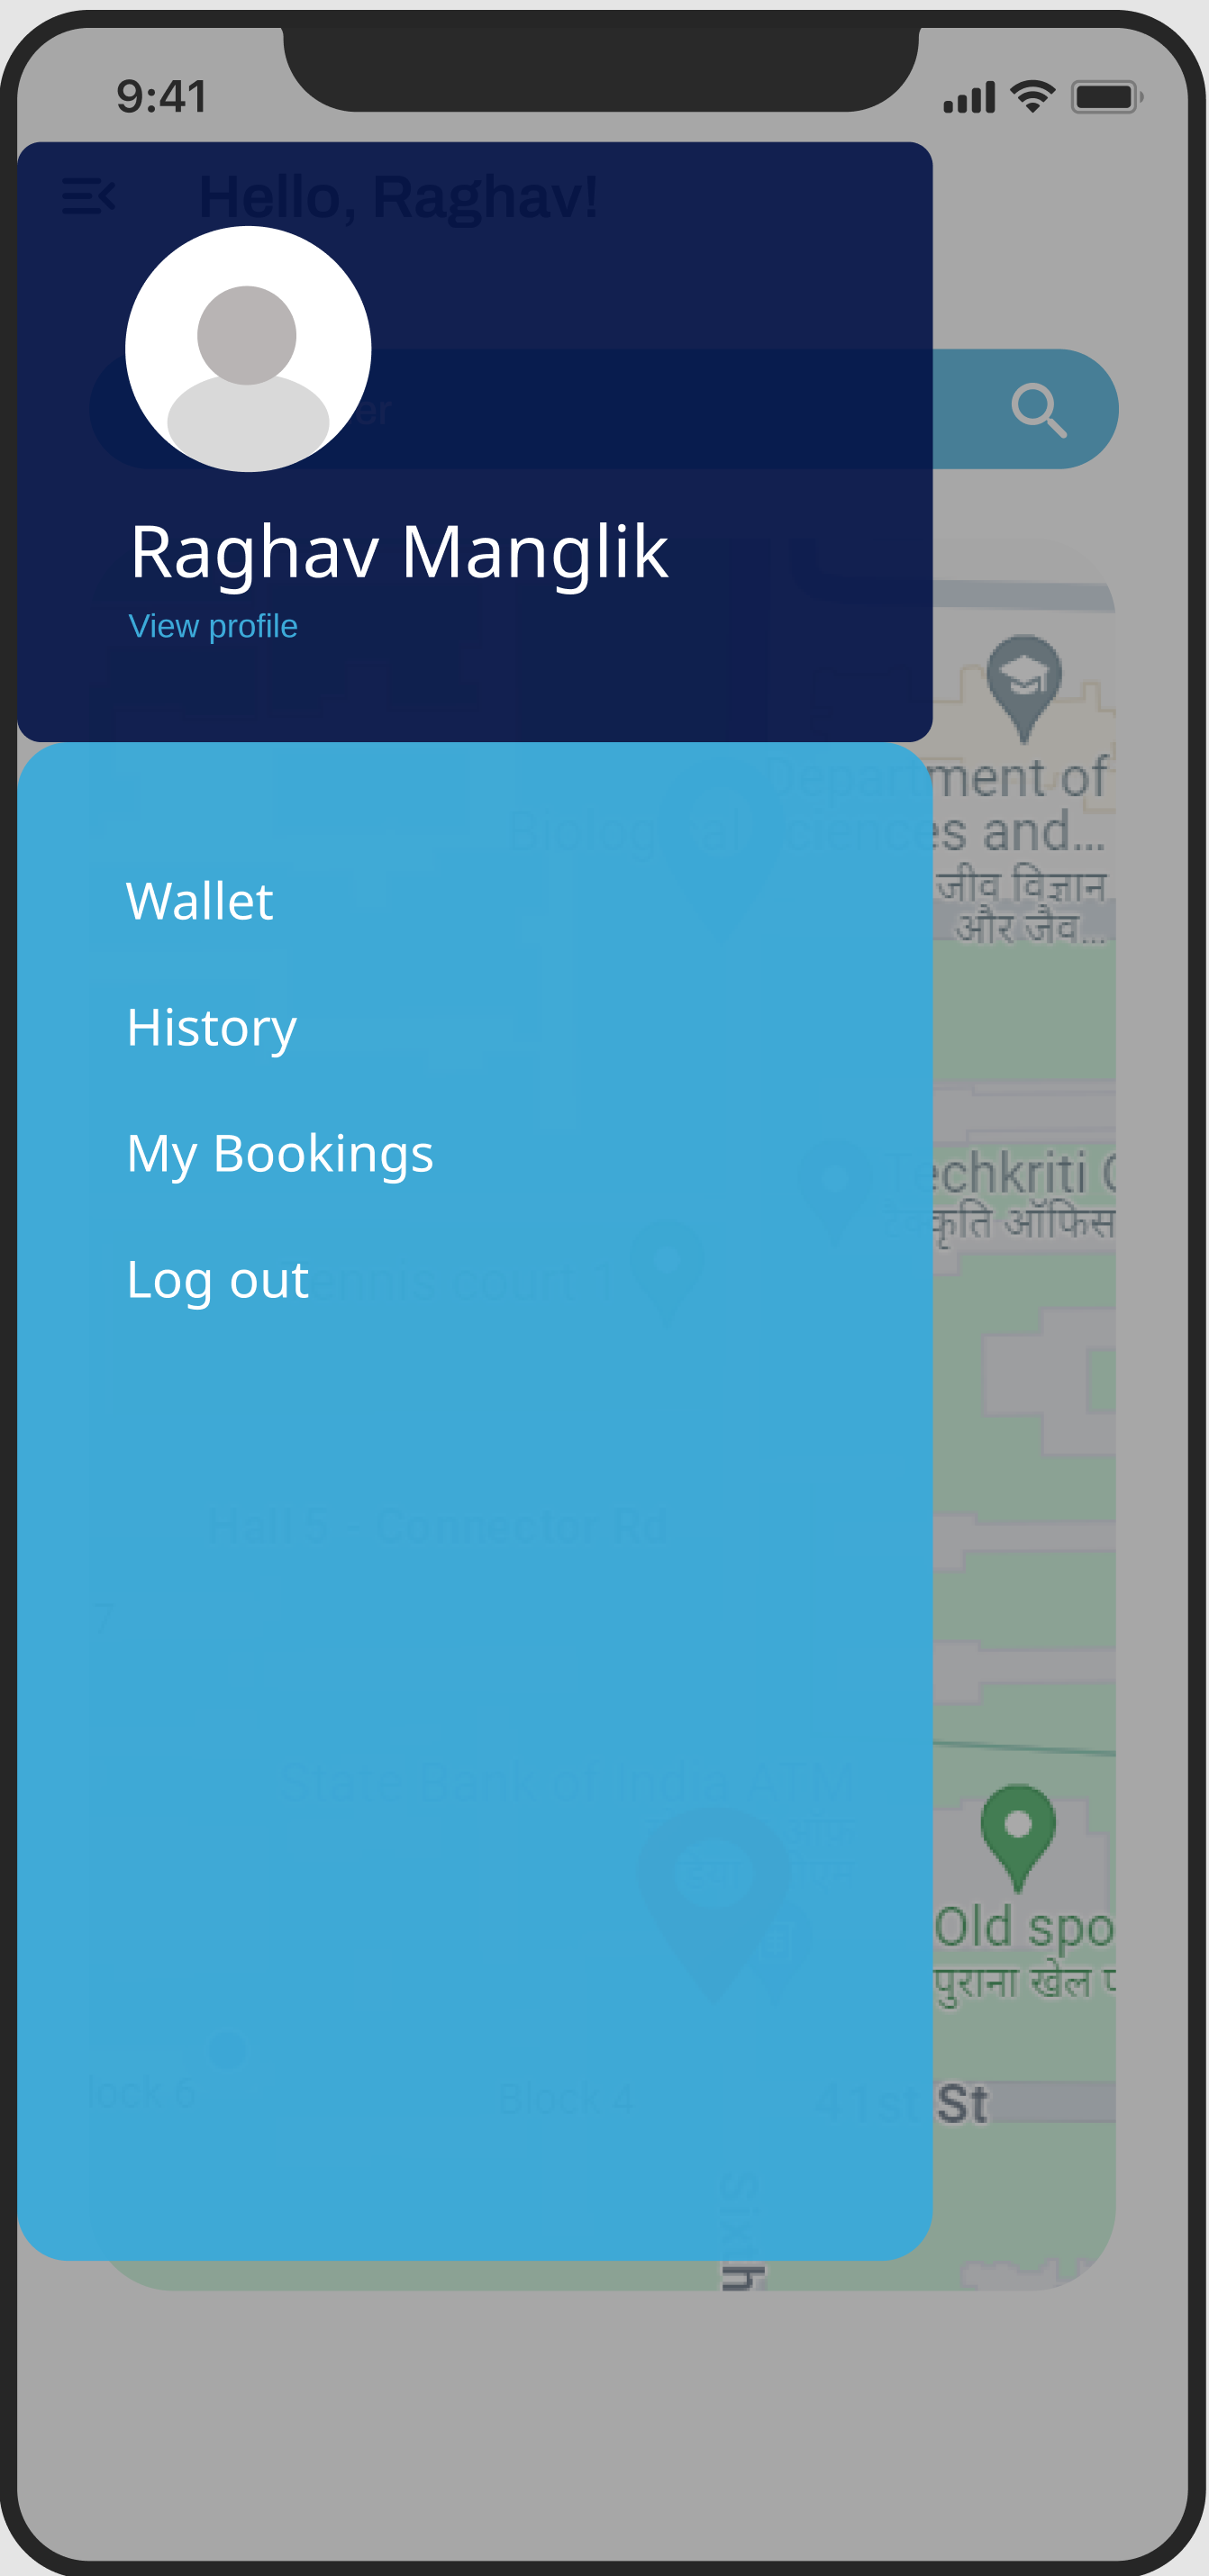
\includegraphics[scale=0.1]{ui-images/Navbar.png} & 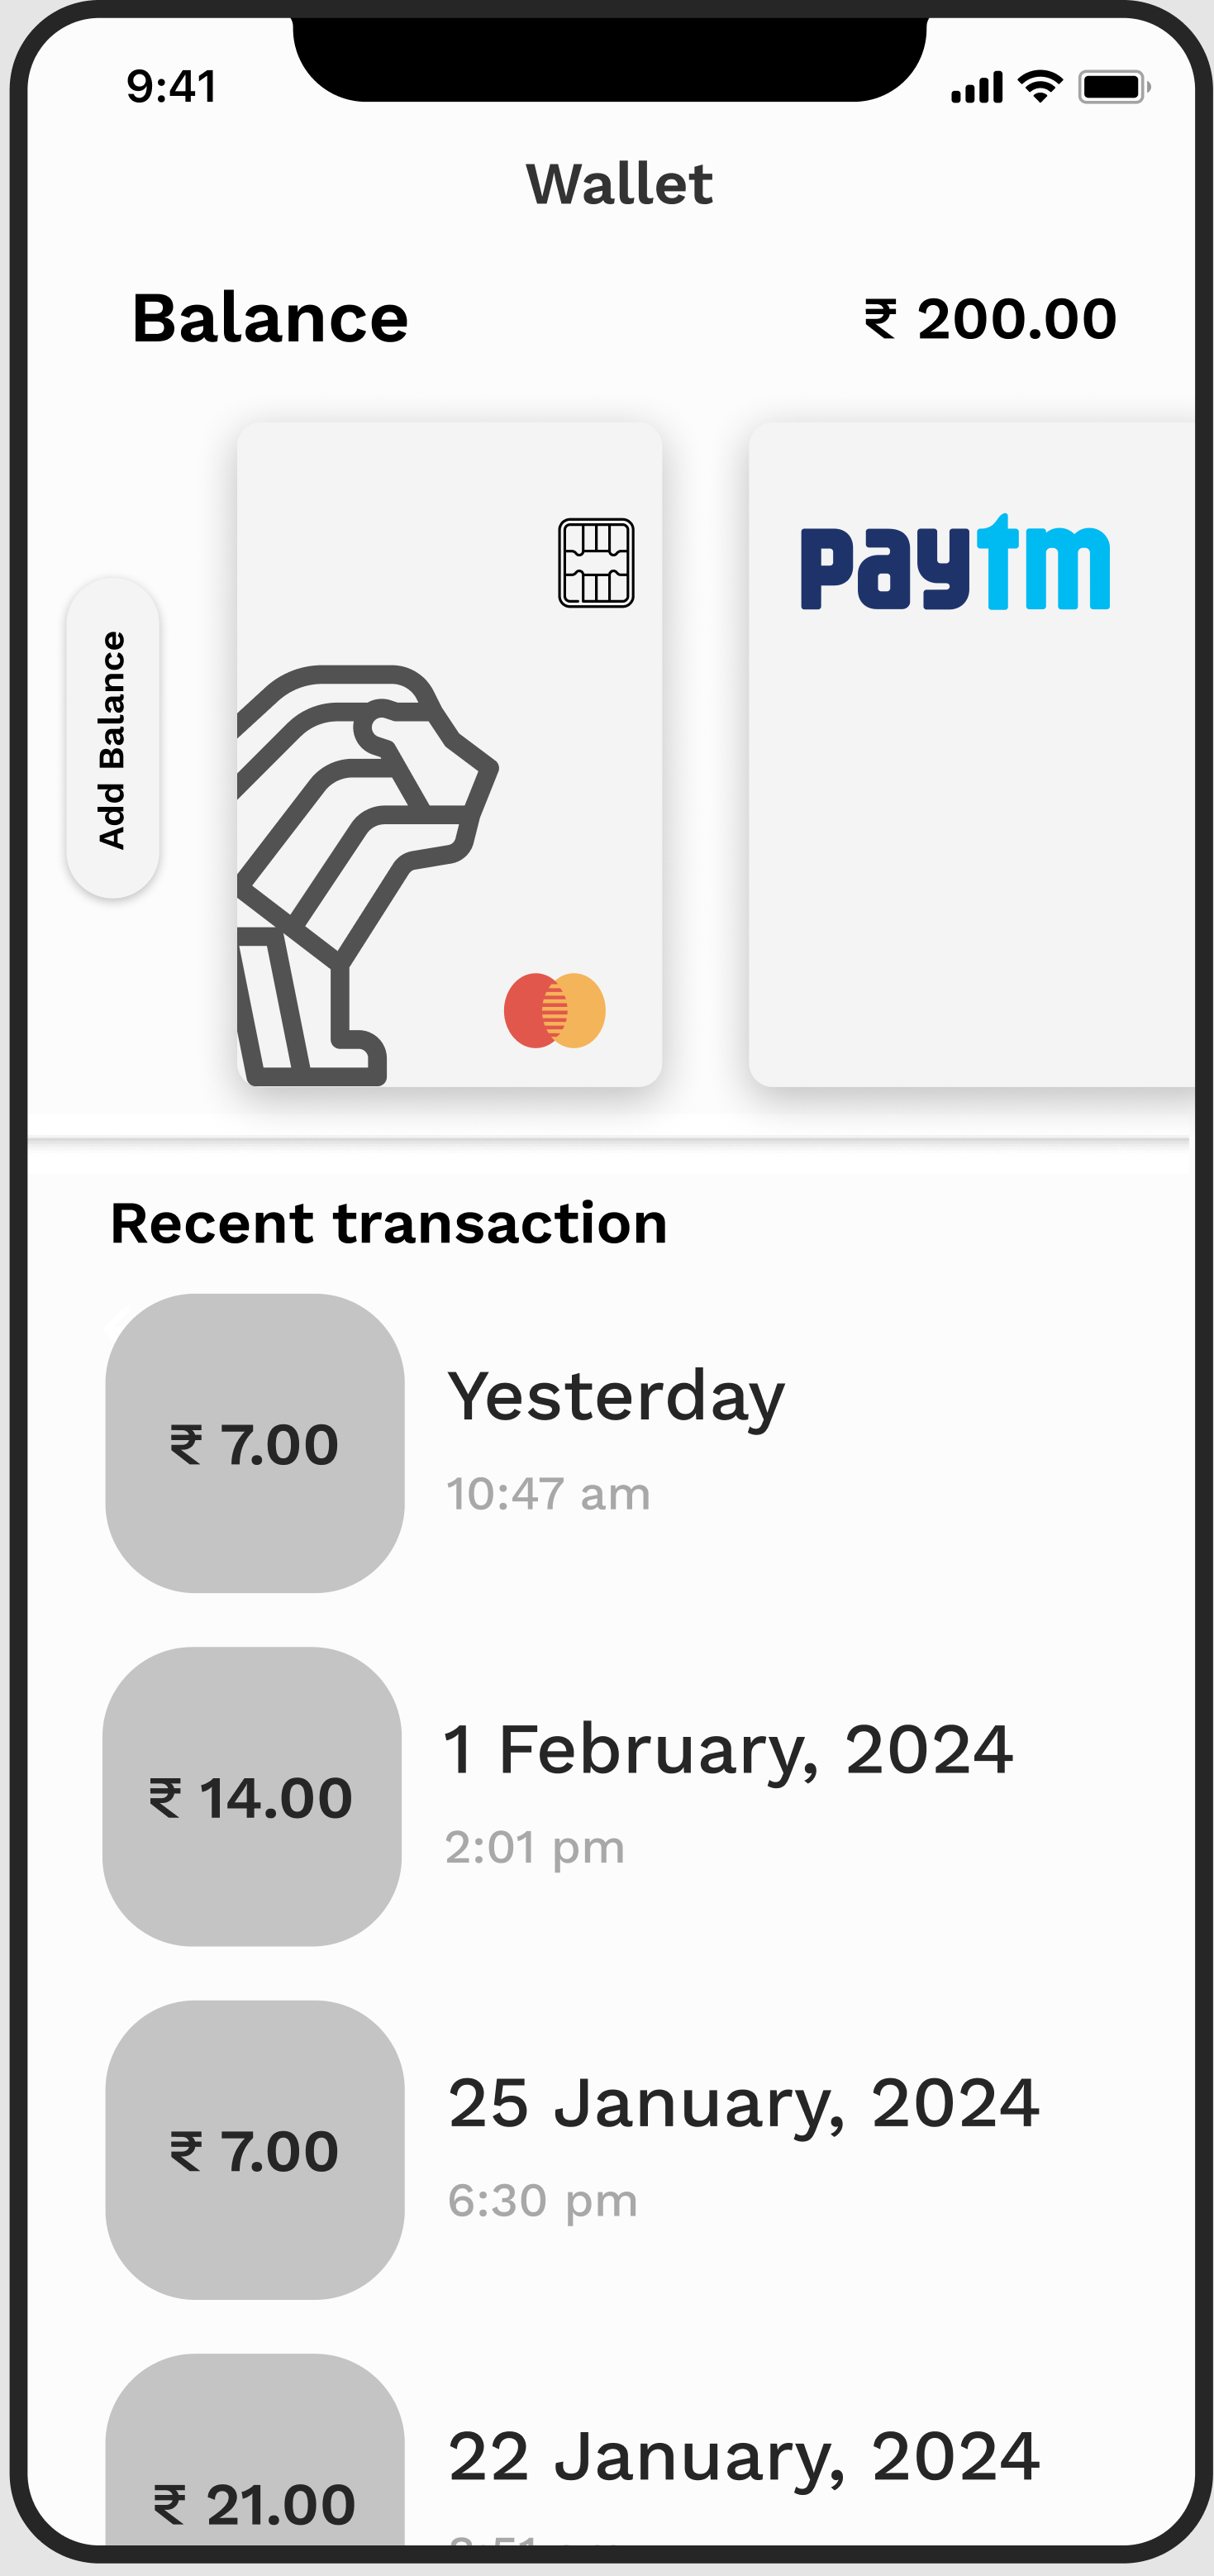
\includegraphics[scale=0.1]{ui-images/Wallet.png} & 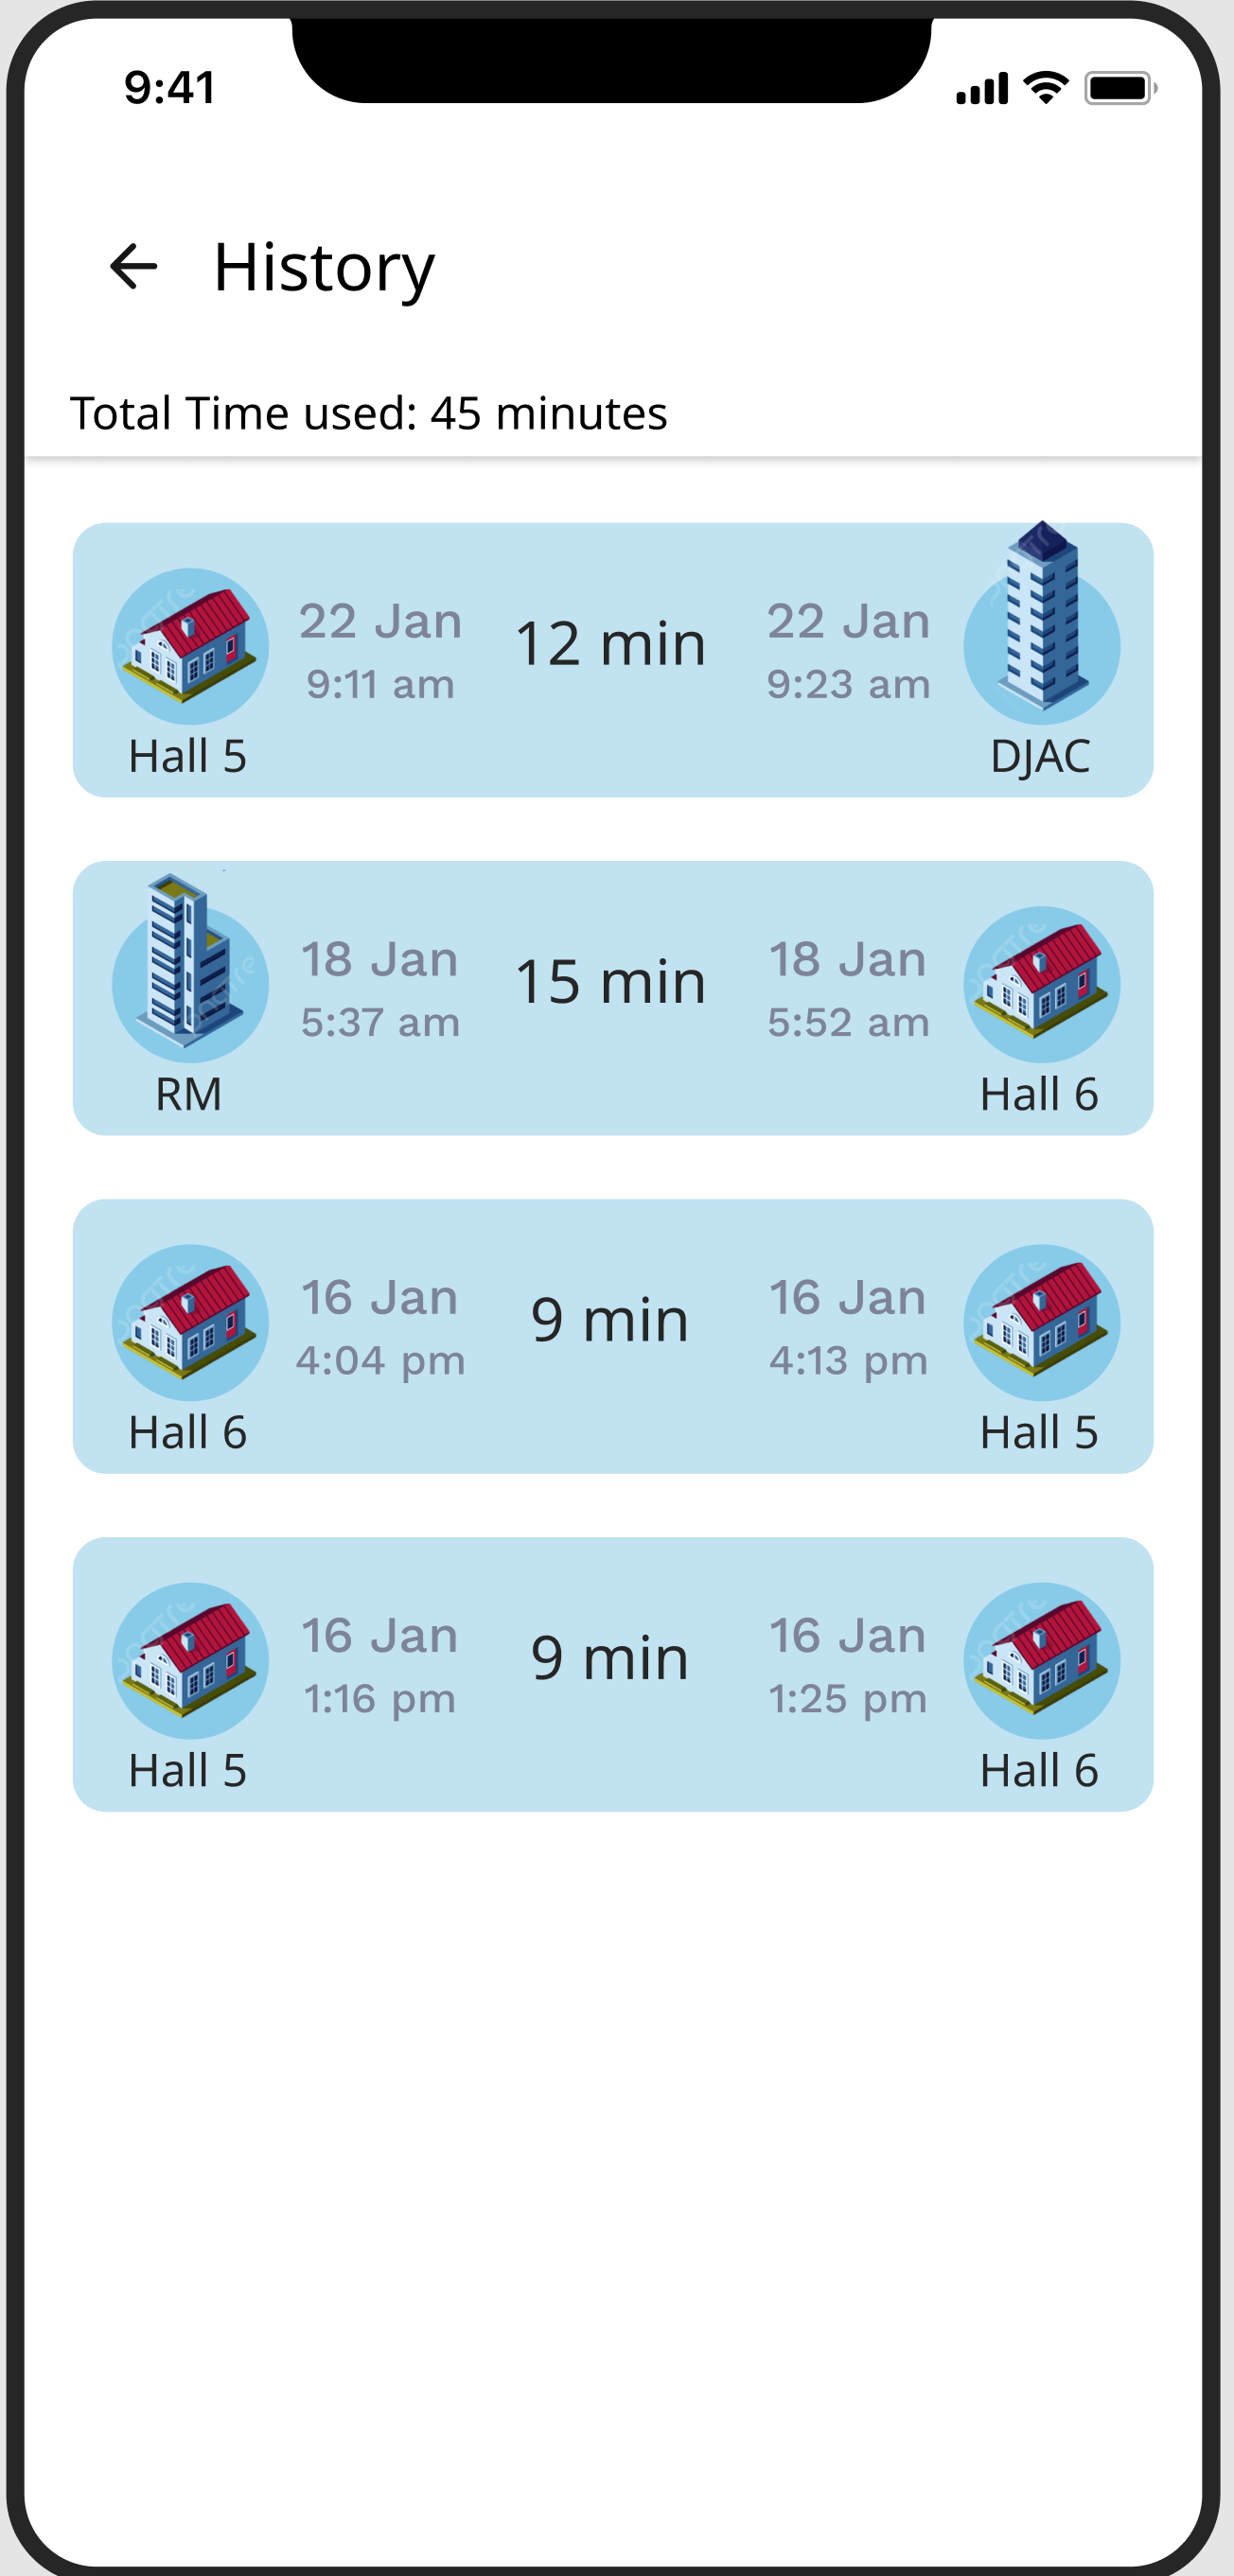
\includegraphics[scale=0.25]{ui-images/History.png}
\end{tabular}


\begin{tabular}{cc}
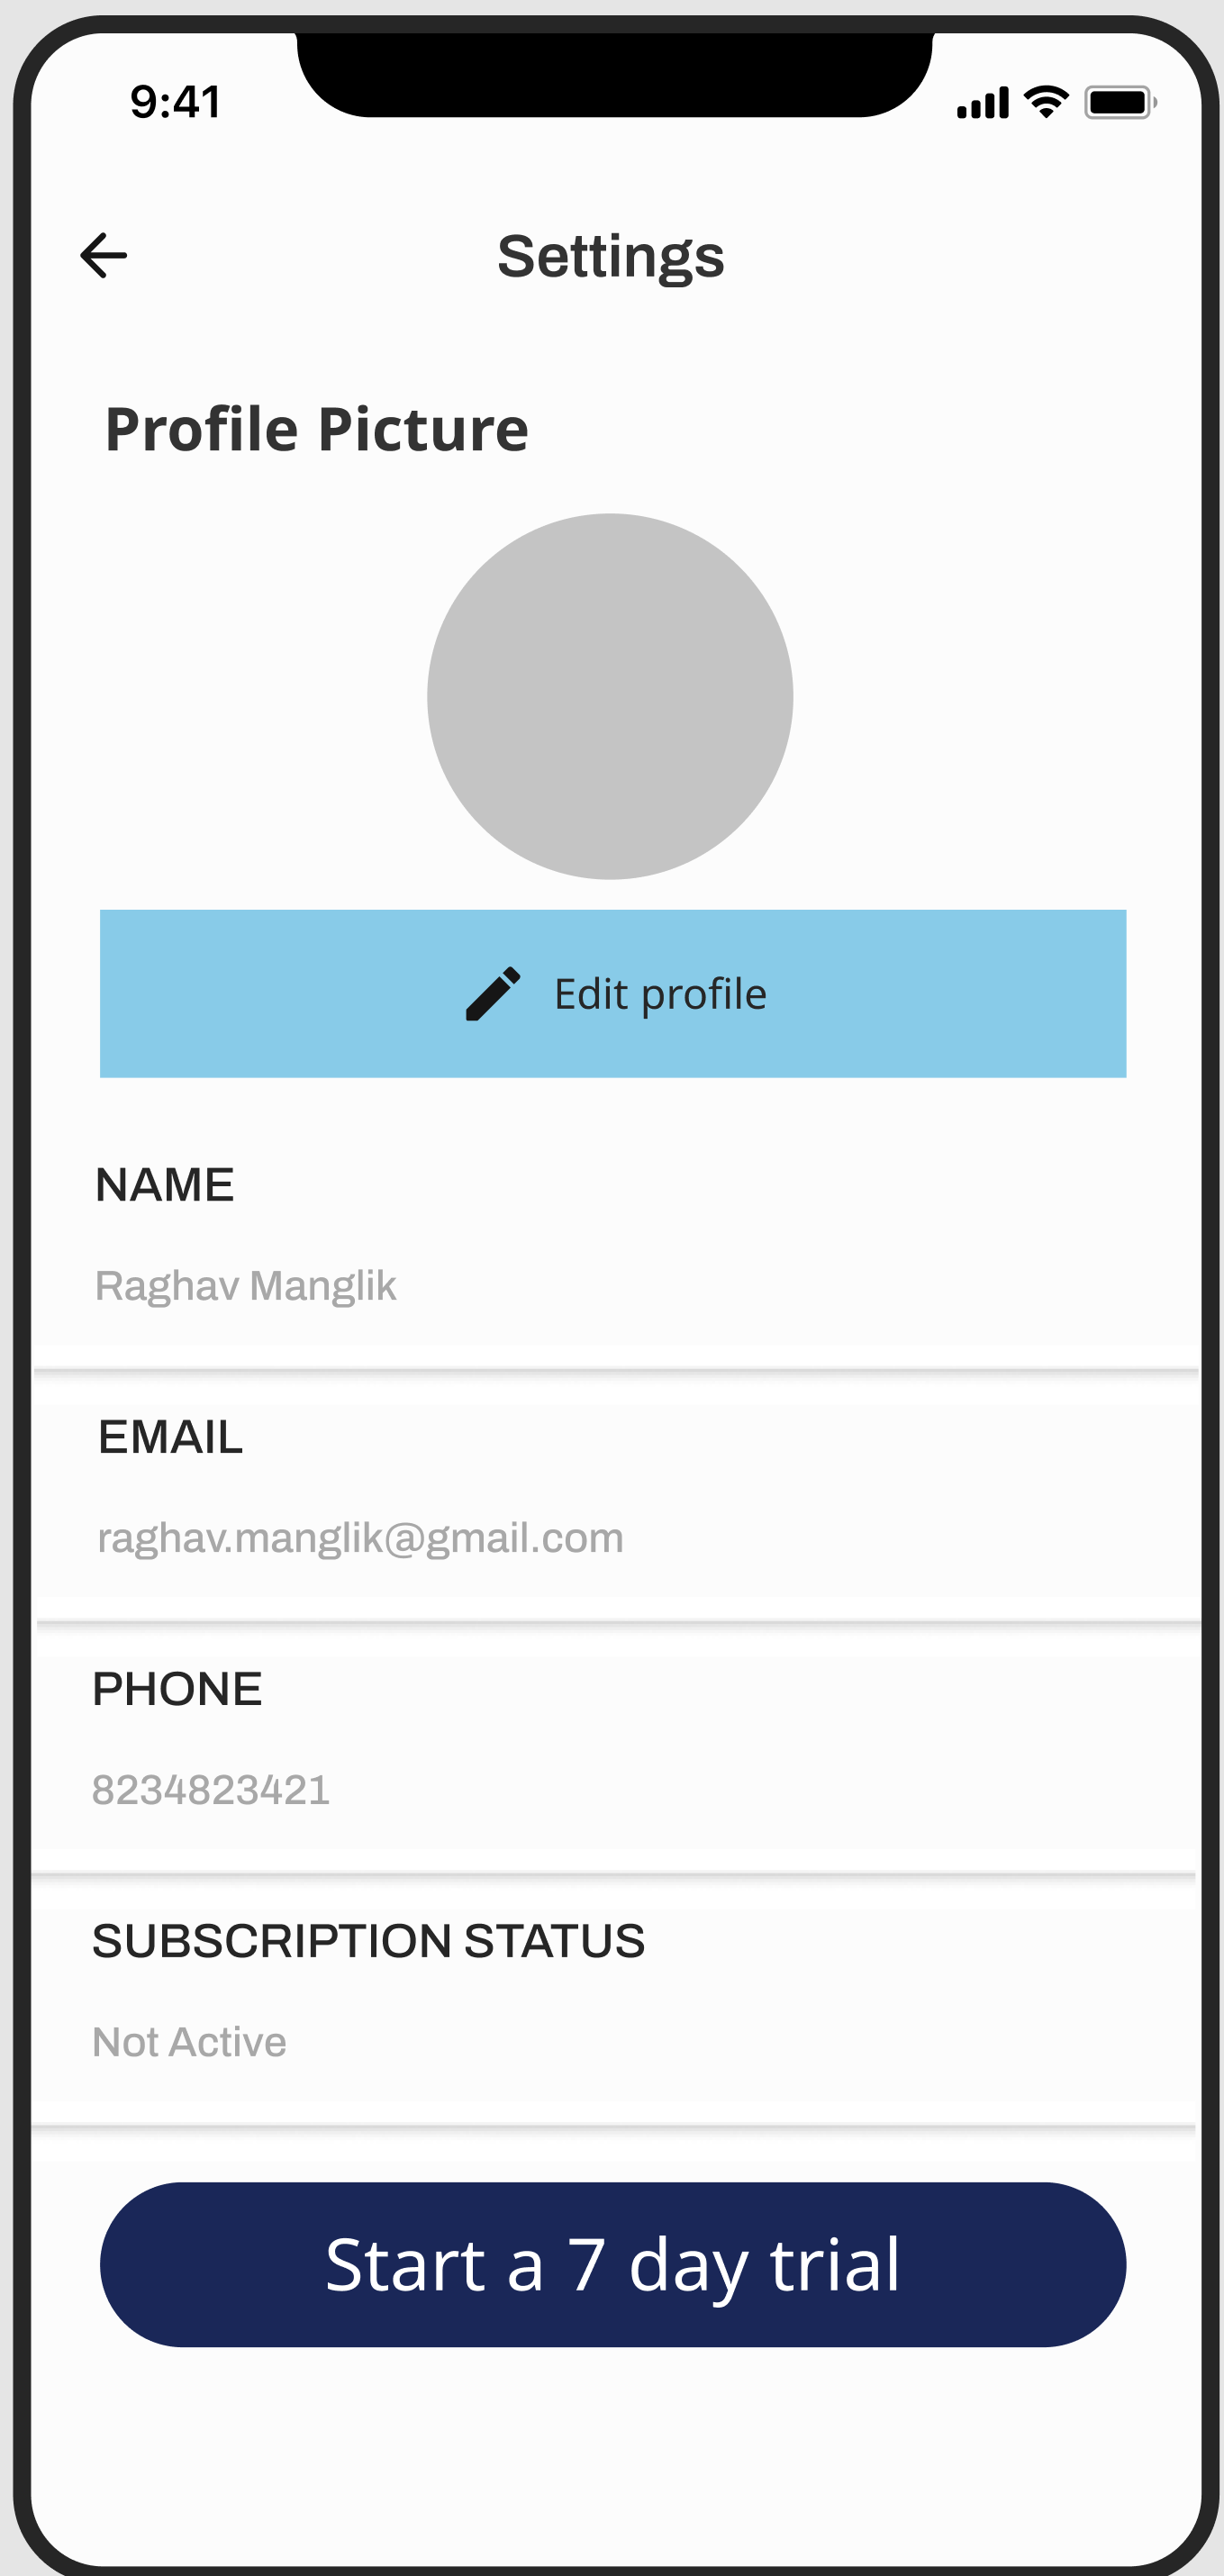
\includegraphics[scale=0.1]{ui-images/Settings.png} & 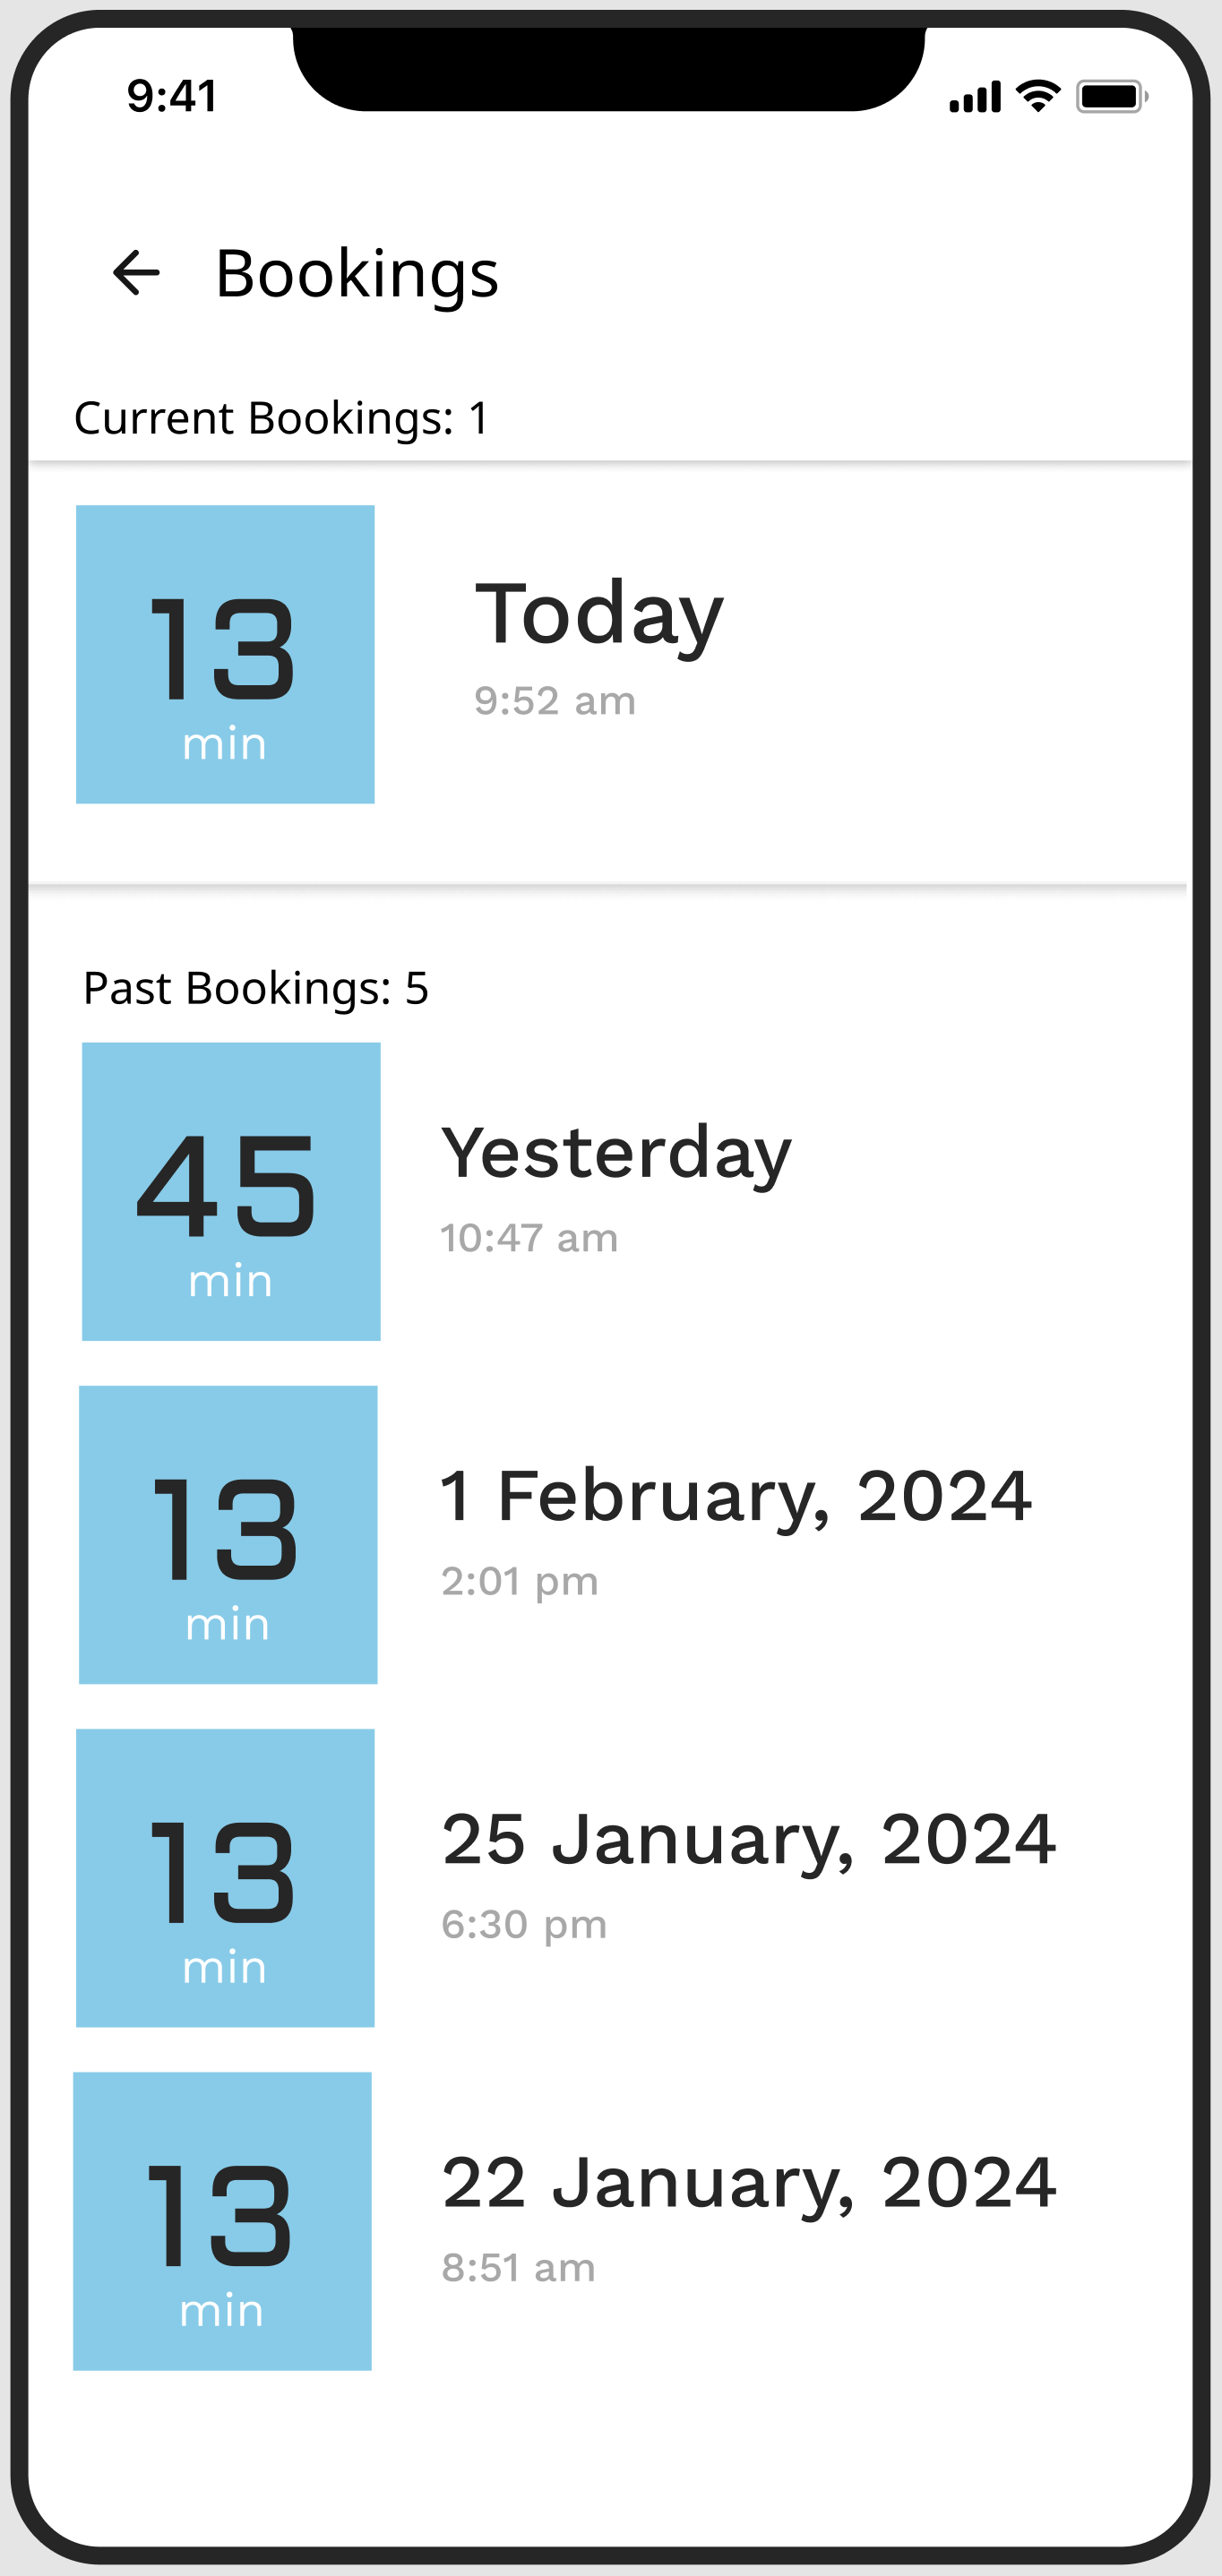
\includegraphics[scale=0.1]{ui-images/Bookings.png}
\end{tabular}
\end{center}

\subsubsection{Admin Interface}
The admin interface is used to manage the hubs and cycles. The admin can add new hubs, view the details of the hubs, and manage the cycles. The admin can also view the feedback and issues reported by the users.
\begin{center}
    \includegraphics[scale=0.08]{ui-images/AdminLogin.png}
    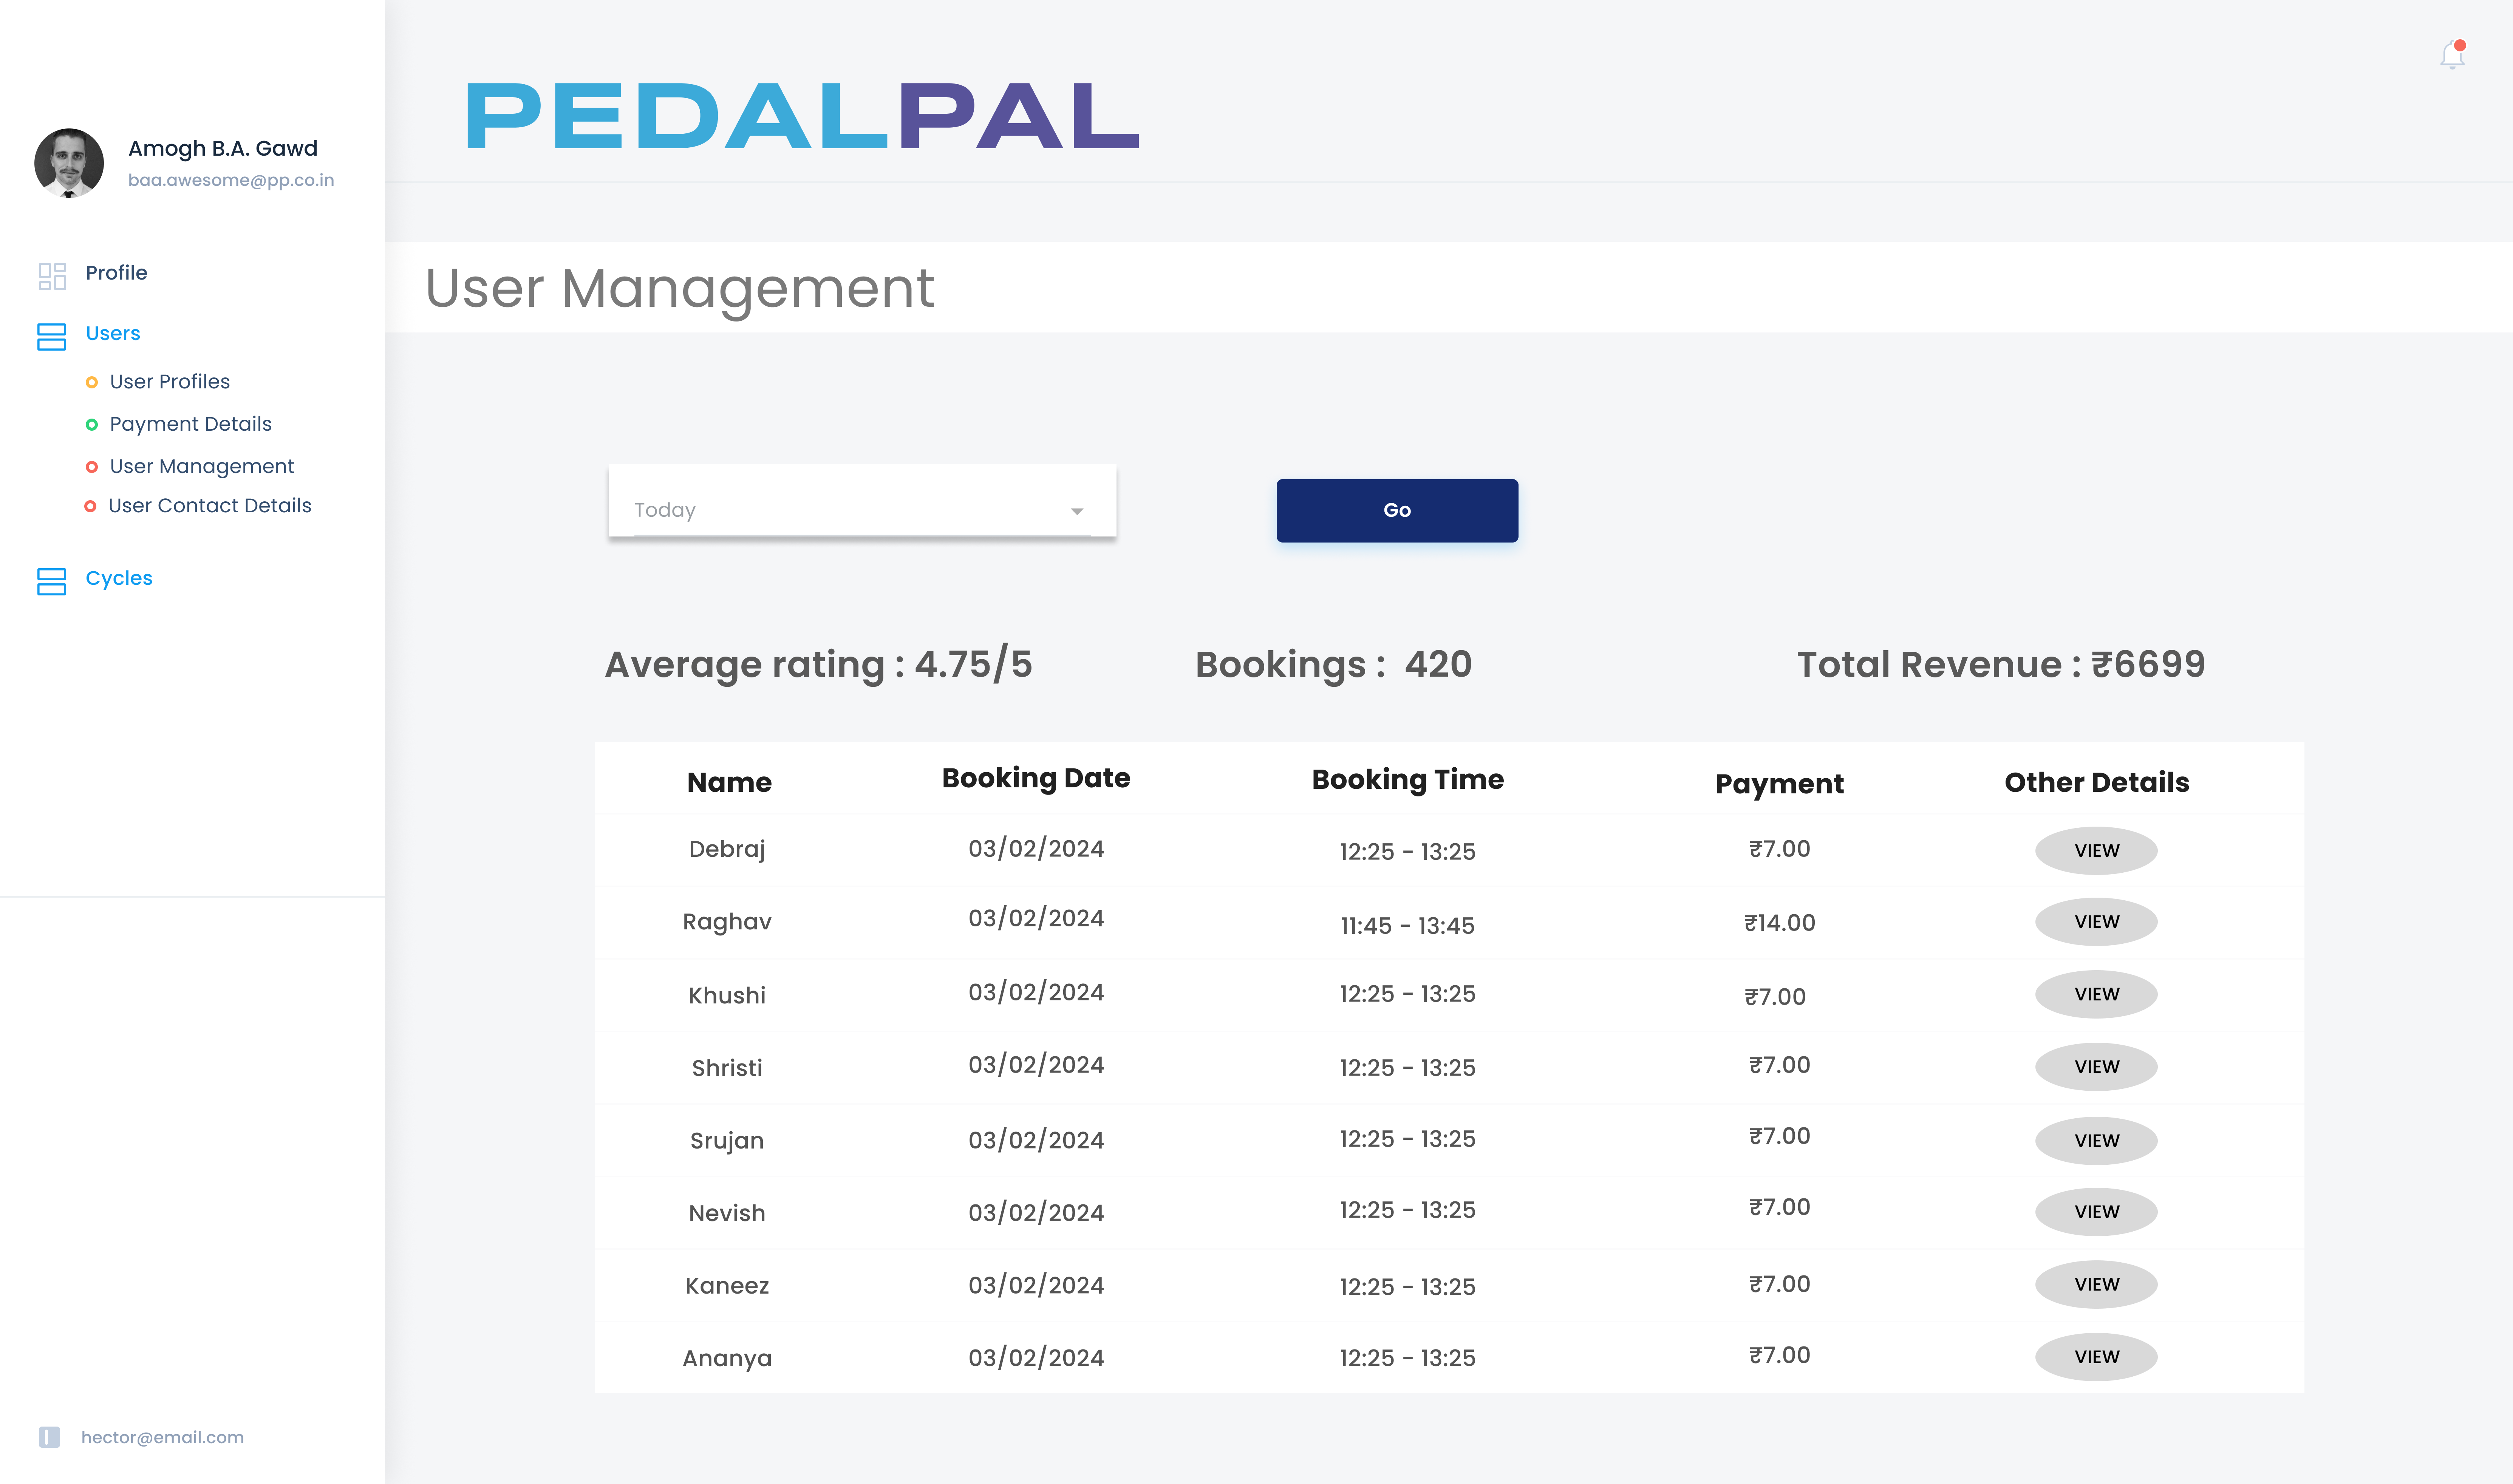
\includegraphics[scale=0.08]{ui-images/AdminDashboard.png}
\end{center}

